\documentclass{article}

\usepackage[paperheight=11in,paperwidth=8.5in,top=1.5in,bottom=1.5in,right=1in,left=1in]{geometry}

\usepackage{url}
\usepackage[latin1]{inputenc}
\usepackage{graphicx}
\usepackage{pdflscape}

%%%%%%%%%%%%%%%%%%%%%%%%%%%%%%%%%%%%%%%%%%%%%%%%%%%%%%%%%%%%%%%%%%%%%%%%%%%%%%
% front page
%%%%%%%%%%%%%%%%%%%%%%%%%%%%%%%%%%%%%%%%%%%%%%%%%%%%%%%%%%%%%%%%%%%%%%%%%%%%%%

\begin{document}

%\begin{frontmatter}


\title{Parallelizing Evolutionary Algorithms on GPUs:\\ Current Trends and Methodologies}

%\author{Gustavo Romero$^1$, M.G. Arenas$^1$, A.M. Mora$^2$, \\
%P. Garc{\'\i}a-S{\'a}nchez$^3$, J. J. Merelo$^1$, P.A. Castillo$^1$  \\ \\
%\small{$^1$ Dept. Computer Architecture and Computer Technology,}\\
%\small{ETSIIT-CITIC, University of Granada (Spain)}\\
%\small{$^2$ Dept. Signal Theory, Telematics and Communications,}\\
%\small{ETSIIT-CITIC, University of Granada (Spain)}\\
%\small{$^3$ Dept. Computer Engineering, University of C{\'a}diz (Spain)}\\
%\small{\texttt{\{gustavo,mgarenas,pacv,amorag,jmerelo\}@ugr.es}}\\ \small{\texttt{pablo.garciasanchez@uca.es}}
%}

\maketitle

%%%%%%%%%%%%%%%%%%%%%%%%%%%%%%%%%%%%%%%%%%%%%%%%%%%%%%%%%%%%%%%%%%%%%%%%%%%%%%
% abstract
%%%%%%%%%%%%%%%%%%%%%%%%%%%%%%%%%%%%%%%%%%%%%%%%%%%%%%%%%%%%%%%%%%%%%%%%%%%%%%

\begin{abstract}
Evolutionary Algorithms (EAs) are the most prolific metaheuristic adapted to General Purpose Graphics Processing Units (GPGPUs), as they are population-based approaches inherently parallel.
Thus, this paper firstly aims to be a tutorial regarding the parallelization of EAs on GPGPUs, introducing their general features and main distributed models, together with several frameworks which allow to conduct this task easily, and the main issues to take into account in order to carry out these parallel implementations.
The work also reviews the new advances in hardware and software in this field.
Finally, the paper presents a deep survey on the literature related to the adaptation of EAs to GPGPUs. Thus, 194 publications have been revised, extracting their key features to categorize them.
We have followed a taxonomy of the approaches used for GPGPU parallelization. Then, a more in-depth analysis has been conducted on the most representative works in each category.
\end{abstract}

%\begin{keyword}
%parallel computation \sep evolutionary algorithms \sep metaheuristics \sep GPUs \sep GPGPUs \sep survey
%\end{keyword}
%
%\end{frontmatter}

%% main text

%%%%%%%%%%%%%%%%%%%%%%%%%%%%%%%%%%%%%%%%%%%%%%%%%%%%%%%%%%%%%%%%%%%%%%%%%%%%%%
\section{Introduction}
\label{sec:intro}
%%%%%%%%%%%%%%%%%%%%%%%%%%%%%%%%%%%%%%%%%%%%%%%%%%%%%%%%%%%%%%%%%%%%%%%%%%%%%%

Evolutionary Algorithms (EAs) \cite{EAs_Back96} are a class of probabilistic search and optimisation methods inspired on the model of Darwinian evolution.
The main features common to all the approaches are a population of individuals or potential solutions for the target problem, a selection method that favours better solutions, and a set of operators that iteratively act upon the selected solutions. If there is defined a correct {\em fitness function}, which assigns a reliable value to every individual, this process guarantees that the average quality of the population will increase with the number of generations.

This metaheuristic has been widely used in the literature to solve many different problems, due to its simplicity and facility to be implemented. However, the application of EAs to find the solution of either real world problems or large instances of some benchmark problems, requires a high amount of computational power. Thus, it is quite frequent to implement a parallel or distributed version of this kind of algorithms.

Even if EAs were proposed as sequential methods, their features, such as the population of independent solutions they manage, or some operators/functions which are applied on every individual at a time, make them intrinsically parallel approaches, and thus, very suitable to be distributed or parallelized (at different grain levels).
The aim of the parallelization is usually the improvement of the running time for yielding an objective solution, if known, or for obtaining a certain degree of quality in the solution, if it is not the optimal. But sometimes this distribution also implies a different searching scheme, which leads to a different searching area of the space of solutions and thus, which yields a different solution or set of solutions for the problem, that could be better than the one obtained in the sequential approach.
For these reasons, EAs are so far the most prolific metaheuristic in
terms of existing parallel approaches, so this survey will be focused on them.

In the last years, new trends in parallelization and
distribution of algorithms have emerged. These are technologies such as Peer-to-Peer (P2P) \cite{P2P-wikipedia}, Service-Oriented Architectures \cite{SOA-wikipedia}, Cloud Computing \cite{CloudComputing-wikipedia}, or Volunteer Computing \cite{VolunteerComputing-wikipedia}, to cite the most relevant. There are several adaptations of EAs to every of them \cite{laredo2010evag,SOA-Garcia-SanchezGCAG13,Meri_CloudEA13,Volunteer-LaredoBGVAGF14},
% Antonio - poner otras citas? Son todas nuestras. :_D
% What about this? - JJ
which involve a new way to develop parallel EAs, taking into account some shortcomings, such as the integration of heterogeneous elements or dynamic resources, and also to deal with fault-tolerance, churn, massive
scalability or decentralization.

Besides, the advances in the video game industry have led to the production of low cost and high-performance graphics processing units (GPUs), which mitigate several of these issues.
GPUs are specialized stream processors, composed of hundreds (or
thousands) of computation units, and designed to perform graphics
manipulations applying optimized graphical primitive operations, at a
much higher speed than a general purpose CPU.

GPUs have been adapted to be used as General Purpose multi-processors
with shared memory, or GPGPUs, in a similar shape to Single
Instruction Multiple Data (SIMD)\cite{SIMD-wikipedia} architectures.
To this end, there are specific programming languages and structures that can be used by developers to write their own programs to be run on a GPU, which are very effective for scientific computing in terms of cost, given their extremely high performance in the comparison with CPU-based computing.
This makes these architectures well suited to run large or complex computational problems in parallel, as substitutes or complements for CPUs, and therefore, GPU-based large-scale systems are appearing \cite{KindratenkoTrends11}.

EAs have also adopted this new trend, and a huge amount of parallel and distributed approaches on GPGPUs have arisen in the last years.
Thus, this paper presents a taxonomy regarding the different
parallelization models, along with a complete survey of the most
relevant proposals in this scope, extracted after revising more than
200 works published since 2004.

In addition, the manuscript introduces the main concepts related with
GPUs, from their internal architecture, to the usual programming
models and structures, through several widely used tools and
frameworks which can help to do this task. After this introduction, the work gives some guidelines to parallelize an EA using GPGPUs, pointing out the main issues and constraints that should be taken into account.

The rest of the paper is structured as follows:
Section \ref{sec:eas} introduces EAs and describes the most usual parallelization and distribution models in the literature.
In Section \ref{sec:parall_and_GPUs}, the internal structure of GPUs
and their utility as GPGPUs are described, as well as a
comparison of the existing cards in the market is shown.
Then, programming schemes, languages and tools used in GPUs are
presented in Section \ref{sec:programming}, followed by a description
of the best frameworks used to parallelize EAs in order to take
advantage of the power of GPGPUs (Section \ref{sec:parallelizing}). In
the same section, the main issues to consider when a parallel version of
an EA wants to be implemented on a GPGPU, are commented.
Next, Section \ref{sec:taxonomy} proposes a taxonomy based on the different parallel models implemented in the literature, in order to categorize the revised papers. Thus, in Section \ref{sec:survey} a set of representative works (according to their number of citations) describing different approaches using GPGPUs are reviewed and divided following the proposed taxonomy, plotting also some interesting numbers and graphs related to them.
Finally, some conclusions are remarked in Section \ref{sec:conclusions}.


%%%%%%%%%%%%%%%%%%%%%%%%%%%%%%%%%%%%%%%%%%%%%%%%%%%%%%%%%%%%%%%%%%%%%%%%%%%%%%%
\section{Evolutionary Algorithms}
\label{sec:eas}
%%%%%%%%%%%%%%%%%%%%%%%%%%%%%%%%%%%%%%%%%%%%%%%%%%%%%%%%%%%%%%%%%%%%%%%%%%%%%%%

This section gives a general overview of the most used types of Evolutionary Algorithms (EAs) describing their common elements. In addition, the most extended models to parallelize EAs are presented, to understand all their possible architectural possibilities.

% ------------------------------------------------------------------------------
\subsection{Description}
\label{subsec:eas-description}

EAs are a set of bioinspired techniques applied to optimization problems \cite{eiben2010whatis}, based on the process of natural selection \cite{darwin1859}. In this kind of pseudo-stochastic algorithms, a \textit{population} of codified solutions (called \textit{individuals}) is created. There is also a \textit{fitness} function, which evaluates the level of adaptation of the individuals to the problem to solve.
Thus, the fittest individuals have more chances to be selected for reproduction, so their offspring could inherit their genetic material.


%\subsection{Types of Evolutionary Algorithms}
%\label{sec:distributed:types}
The general scheme of an EA, extracted from the work by Eiben and Smith \cite{eiben2010whatis} is described in Figure \ref{fig:basicscheme}.

% There is a nicer "Algorithmic" package. Use it - JJ
\begin{figure}[tb]
\begin{verbatim}
BEGIN
 INITIALISE population with random candidate solutions;
 EVALUATE each candidate;
 REPEAT UNTIL (TERMINATION CONDITION is satisfied) DO
   1 SELECT parents;
   2 RECOMBINE pairs of parents;
   3 MUTATE the resulting offspring;
   4 EVALUATE new candidates;
   3 SELECT individuals for the next generation;
 OD
END
\end{verbatim}
\caption{General scheme of an evolutionary algorithm in pseudo-code, obtained from \cite{eiben2010whatis}.}
\label{fig:basicscheme}
\end{figure}

Although most of the EAs follow this structure, there are some differences depending on the representation of solutions, the operators to apply, or even the kind of problem to solve. Thus, according to Eiben \cite{eiben2010whatis}, the classical types of EAs are:

%A possible classification is presented in this section, taking into account the new approaches that cannot fit with the traditional taxonomy. This classification would help to clarify the elements that  distinguish an algorithm from another (for example, the operators), and the existing similarities and differences, in order to establish a good starting point to classify EAs in GPGPUs.

%\subsection{Classic classification of EAs}
%\label{subsec:classicEAs}
%EAs are usually classified using a traditional variant, according to
%the book of Eiben and Smith \cite{eiben2003introduction}. These authors clarify that the features of an EA are:
%\begin{itemize}
%\item EAs are population-based.
%\item EAs mostly uses recombination to generate new individuals from the existing ones.
%\item EAs are stochastic.
%\end{itemize}


\begin{description}
\item [Genetic Algorithms] These kind of algorithms were initially proposed by Holland \cite{holland1975adaptation}, and later revised by Goldberg \cite{goldberg1988genetic}.
In this kind of EA, the representation of the solution is a string of numbers (normally binary), called \textit{chromosome}. The individuals are selected proportionally to their fitness, and then different \textit{recombination} and/or \textit{mutation} operators are applied to generate new individuals that will be included in the population (replacing some other). %These algorithms have been used in different areas, such as function optimization \cite{michalewicz1996genetic}, combinatorial optimization \cite{Esparcia2009EVITA}, artificial intelligence in videogames \cite{Fernandez20111optimizing}, or generative art \cite{Garcia2013RGB}, among others.

\item[Evolution Strategies] The Evolution Strategies (ES) are applied to solve problems whose solution is included in the domain of real numbers. Their main difference with GAs is the consideration of a self-adaptation of the mutation rate, being coded in each individual \cite{eiben2005shared}. In addition, the parent selection is conducted randomly, instead of being based on the fitness. %ES have been applied in fields such as Evolutionary Robotics \cite{Garcia2012testing}.



\item[Genetic Programming] The objective of this technique is to
  generate (and evolve) functions or programs to solve specific
  problems. Each individual is represented in the form of a tree,
  composed of operators (or {\em primitives}) and variables ({\em
    terminals}). These sets are usually fixed and known in advance.
  The genome size is, therefore, variable, but there is frequently a maximum size for the individuals, in order to avoid too high evaluation costs. %GP has been used to evolve LISP (LISt Processing) programs   \cite{Koza1990Tools}, or XSLT (eXtensible Stylesheet     Language Transformations) scripts \cite{Garcia2008XSLT}, among  others.

\item[Evolutionary Programming] In Evolutionary Programming (EP), the representation of every solution depends on the nature of the problem being solved, for example, neural networks \cite{Wang18NeuralNetworks} or Radial Basis Functions (RBFs) \cite{Gonzalez2003multiobjective} have been used as individuals. Another big difference is that is mainly based on self-adaptive mutation, and not in crossover, for individual variation.

  %Don't see a point in making distinctions between these
  %algorithms. They are pretty much the same: population with
  %population-level and individual-level operators. Parallel
  %algorithms won't care if it's GP or GA. Besides, GP and GA are only
  %different with respect to the data structure used - JJ
% Antonio - The idea is just to present EAs and the main types to the reader, regardless their parallelization, it's just an introduction to let him/her understand what is a GA, GP or EP when we mention them later in the text.
\end{description}

%\subsection{Other models}

However, there are other EAs that do not match in the previous
classification. For example \textit{Differential Evolution} (DE)
\cite{storn1997differential}, \textit{Estimation of Distribution
  Algorithms} (EDAs) \cite{larranaga2002estimation} or
\textit{Bayesian Optimization Algorithms} (BOAs)
\cite{pelikan2005bayesian}. DE \cite{storn1997differential} also
exploits a population of potential solutions. Three individuals are
selected randomly from the population to create \textit{random noisy
  vectors}. These vectors are recombined with the initial random
individuals to create the \textit{trial vectors}. They are compared
one by one with the original vectors and the best of each comparison
is kept for the next generation. In the case of EDAs
\cite{larranaga2002estimation}, instead of directly codifying the
variables to optimize, the algorithm tries to find the probability
distribution of each one. In each generation, the individuals are
generated from previous individuals probability distributions. BOA
\cite{pelikan2005bayesian} are based in the creation of Bayesian
networks to generate the offspring from a set of promising
individuals. % So what? If they are not going to be parallelized, why
             % mention them? Just say the basic features you need in
             % al algorithm to be parallelized - JJ
             % Antonio - again, the aim is just to give an introduction


Table \ref{tab:summaryEAs} shows the main differences between all
these types of EAs. Note that we have selected the common features of
each algorithm, but also their typical configurations. For example,
the replacement in GAs can be different from the generational one, or
the representation can also be a real-value vector.
% This is relevant for what? - JJ
% Antonio - for the same reason as before

\begin{table}
  \centering
\begin{tabular}{|p{2.2cm}|p{2.1cm}|p{2.1cm}|p{2.1cm}|p{2.1cm}|p{2.1cm}|}
\hline
				& GA 	 & ES  & EP & GP & DE  \\
\hline\hline
Representation  & Usually finite alphabet strings & Real-value vectors  & Problem-dependent			& Tree 				         & Real-value vectors 	 \\ \hline
Initialization  & \multicolumn{5}{c|}{Usually random, and depending on the problem and individual structure} 						 \\ \hline
Selection 	    & Fitness proportional 	          & Deterministic	      & Tournament-based       & Fitness proportional & Random to create noisy vectors \\ \hline
Recombination   & Genome crossover		            & Genome crossover		& Typically not used	  & Sub-tree exchange		 & Random gene by gene			\\ \hline
Mutation  		 & Random 				                  & Gaussian perturbation	& Gaussian perturbation& Random 				       & Implicit in the noisy vectors	 \\ \hline
Replacement		 & Generational	                    & ($\mu,\lambda$) or ($\mu + \lambda$) survivor selection & 	($\mu + \mu$) survivor selection    & Generational 			   & Compared with the original \\
\hline
\end{tabular}

\caption{Differences between the types of EAs \cite{eiben2010whatis}. These are the typical design choices, but they can vary depending on the problem to solve.}
\label{tab:summaryEAs}
\end{table}




% ------------------------------------------------------------------------------
\subsection{Parallel and Distributed Evolutionary Algorithm Models}
\label{subsec:eas-distributed:parallel}

EAs are inherently parallelizable, since each individual can be
considered in many senses as an independent unit \cite{Alba13parallel}.
% That's not really true... You need several individuals for most operations - JJ
% Antonio - True. Fixed
There are several possible ways to parallelize them: for example, fitness evaluation can be conducted in several slave machines, or the population can be distributed among different nodes to be evolved at the same time.

Two main types of parallelization models for EAs were classified by Alba and Tomassini in \cite{Alba02Parallelism}: \textit{Global parallel EAs} and
\textit{Spatially structured EAs}. This classification is still the
most widely extended, even if it was established in 2002; however, it
does not consider issues such as fault-tolerance, churn, massive
scalability or decentralization. The number of computational nodes are
considered constant during the whole execution and both the network
and the nodes are reliable and trustworthy.

However, with the advent of new technologies, new evolutionary approaches have been proposed that take into account, for instance, the unreliability of millions of nodes co-operating in P2P networks \cite{laredo2010evag}, the data-intensive computing frameworks used in cloud computing \cite{VermaCloud10}, or even in specific informal environments such as distributed file systems or databases \cite{Meri_CloudEA13,Merelo_Couch13}.

On the other hand, since a GPGPU is a kind of
stable and reliable architecture, we consider the classification also
as valid for the purposes of this paper. We will present these
parallelization modes below.

% ----------------------------------------
\subsubsection{Global parallel evolutionary algorithms}
In this model, also called \textit{Farming model},
\textit{Master-Slave} or \textit{Centralized EA}, the parallelism is
applied at evaluation level. Thus, a central node coordinates several
slave nodes. This node executes the EA in a sequential way, but it
distributes the individuals of the population among the slaves just
for being evaluated. Figure \ref{fig:serverClient} depicts this
approach.

\begin{figure}[tb]
\centering
%\includegraphics[width=20pc]{gfx/distributed/serverClient.jpg}
\includegraphics[width=20pc]{serverClient}
\caption{Master-slave model.}
\label{fig:serverClient}
\end{figure}

% ----------------------------------------
\subsubsection{Spatially structured algorithms}
In this scheme the parallelism is performed at population level, that is, the population is divided and distributed among the different computing elements. Depending on how the distribution is performed there are:

\begin{description}
\item[Coarse-grained approach] In which independent subsets of individuals are considered. One of the most extended approaches is the \textit{Island model}, where a number of nodes execute simultaneously the EA, working with different sub-populations at the same time. Each certain number of generations some individuals are interchanged (migrated) between populations. Figure \ref{fig:ring} shows this model with a ring topology.

\begin{figure}[tb]
\centering
%\includegraphics[width=20pc]{gfx/distributed/ring.jpg}
\includegraphics[width=20pc]{ring}
\caption{Island model scheme using a neighbourhood ring topology.}
\label{fig:ring}
\end{figure}

\item[Fine-grained approach] In this approach, also called \textit{Cellular EA} (CEA) \cite{alba-cellular-2008}, each node has one individual of the population, and selection and reproduction are limited to the individuals on the neighbourhood of every node. Usually a bi-dimensional grid is used as topology, such as the one shown in Figure \ref{fig:cellular}.

\begin{figure}[tb]
\centering
%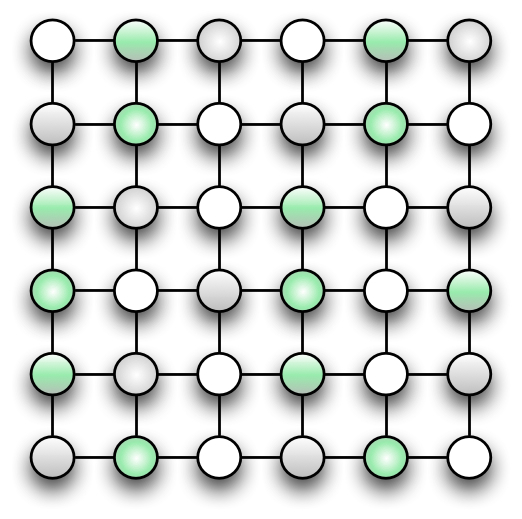
\includegraphics[width=5cm]{gfx/distributed/cellular.jpg}
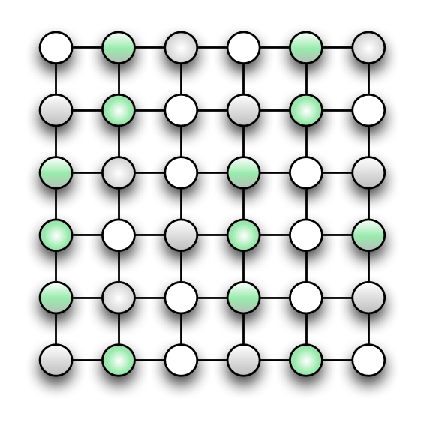
\includegraphics[width=15pc]{cellular}
\caption{Cellular Evolutionary Algorithm.}
\label{fig:cellular}
\end{figure}

\end{description}






%%%%%%%%%%%%%%%%%%%%%%%%%%%%%%%%%%%%%%%%%%%%%%%%%%%%%%%%%%%%%%%%%%%%%%%%%%%%%%%
\section{Massive parallelization on General Purpose GPUs}
\label{sec:parall_and_GPUs}
%%%%%%%%%%%%%%%%%%%%%%%%%%%%%%%%%%%%%%%%%%%%%%%%%%%%%%%%%%%%%%%%%%%%%%%%%%%%%%%

As Gordon Moore predicted in 1965 the number of transistors placed on
integrated circuits has doubled approximately every two years. % This
                                % is not the place to say
                                % this. Probably in the intro - JJ
Obviously this growth rate is not going to be keep into an indefinite future. This trend has been true until the last decade and now it seems to be replaced by Koomey's Law \cite{10.1109/MAHC.2010.28}. It is the equivalent speaking about energy consumption: energy efficiency is doubled every 18 months. For a fixed computation, the amount of battery needed will fall by a factor of two every year and a half. That is, as the primary factor influencing the limits of improving single-node performance is the energy efficiency, new heterogeneous architectures have emerged in response to those limits \cite{VetterHeterogeneous11}.

Parallel computation has passed from been an utility to a
necessity. As newer processors are barely faster than previous ones
the only way to take advantage of the amount of transistors is putting
many cores together. For many year, clock rates and instruction-level
parallelism has become fast enough to allow faster execution of the
same payload on a new processor without modification. Adding heat to
this equation has finally forced chip makers to favor multi-core
designs. Now the only way to benefit from many cores is multi-threaded
software \cite{6307773}.

At the same time graphics card have evolved from small and simple
devices composed of weak arithmetic and logic units to powerful, and
almost general-purpose devices. Earliest academic work about general
computation on GPUs date back to 2002 at the University of Washington
\cite{Thompson:2002:UMG:774861.774894}, and 2004 in Stanford
\cite{Buck:2004:BGS:1015706.1015800}. % so... - JJ

GPUs and CPUs are similar in many ways but there is one key
difference: the philosophy of how to execute a workload. The main
design purpose of a CPU is the fast execution of a single thread of
code. GPUs, on the other side, pursue to maximize the throughput of
multithreaded streams of instructions and data. This is just the
opposite of CPUs. Another difference is the scheduling of threads. For
CPUs, the operating system schedule threads over free cores in a
competitive way. GPUs does it cooperatively with the help from
dedicated hardware. Some of this characteristics can be deduced from
Figure \ref{fig:cpu-gpu}.

\begin{figure*}[!ht]
\centering
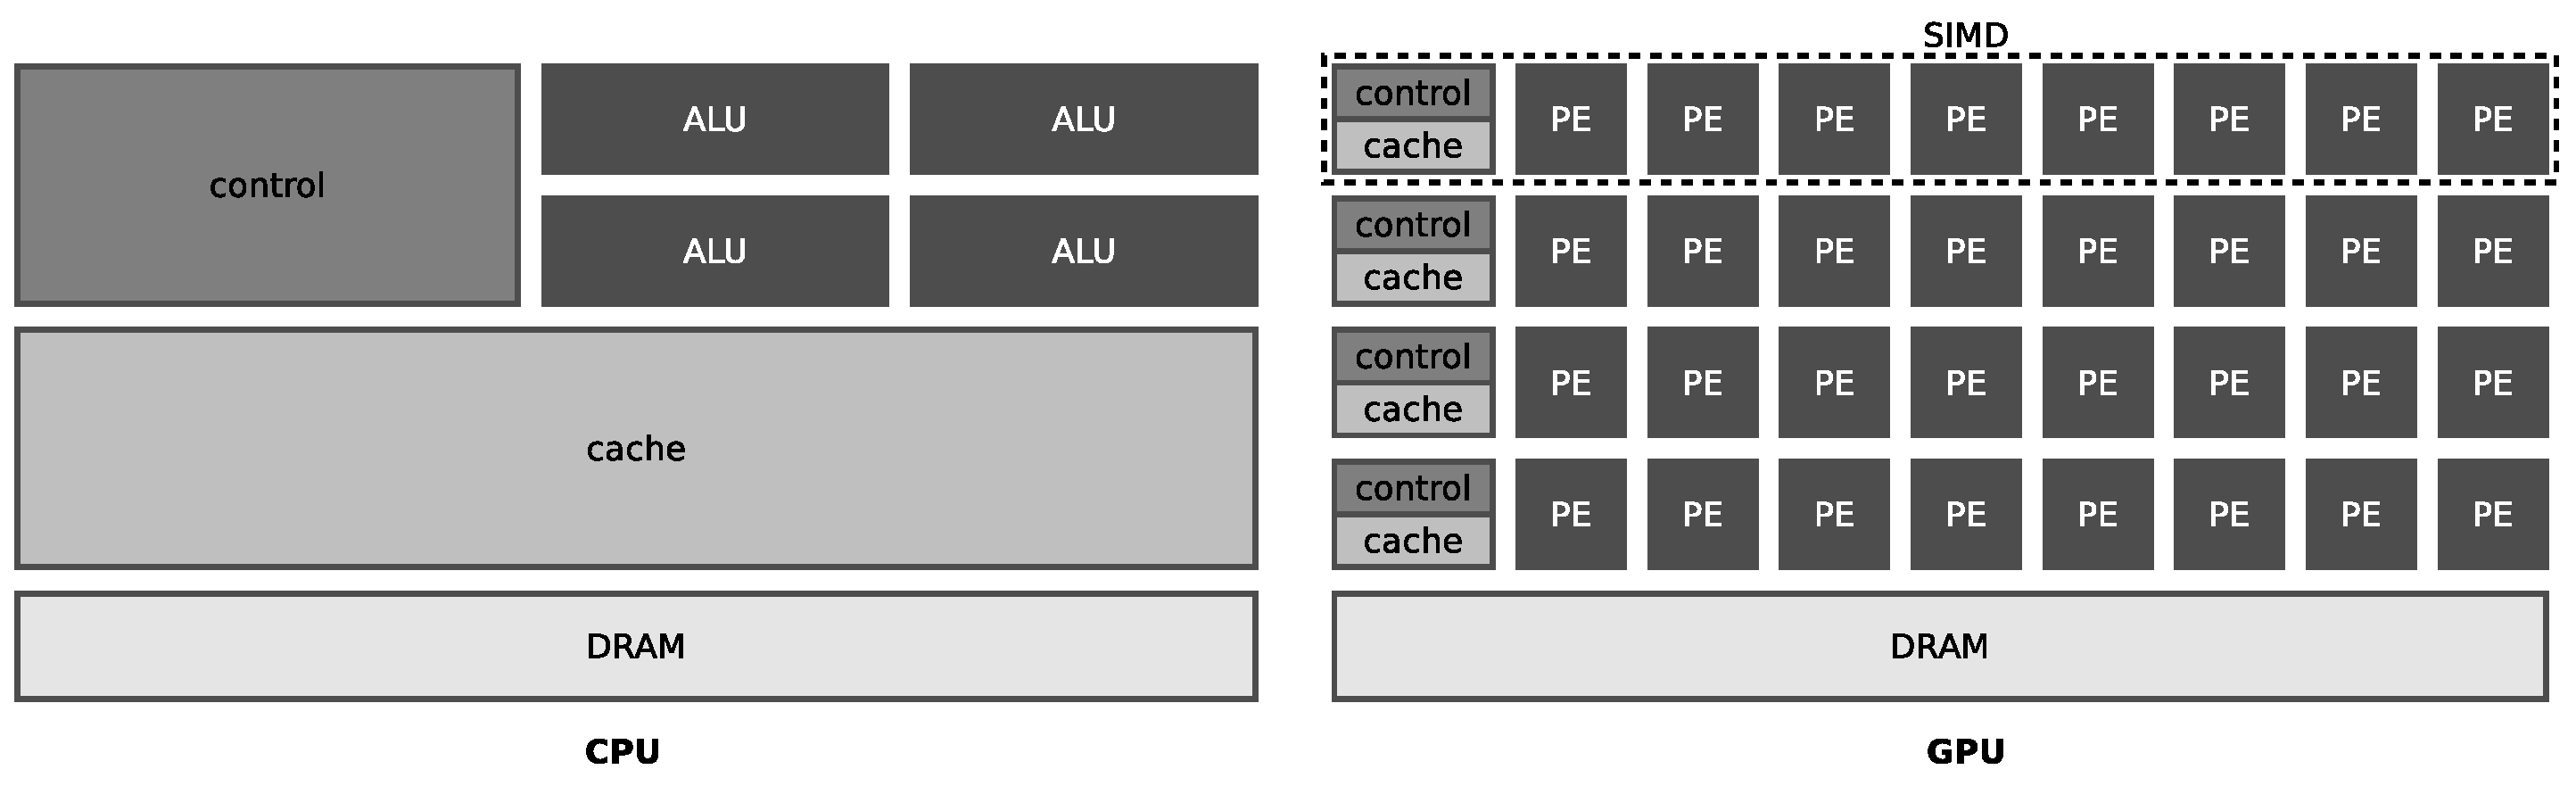
\includegraphics[width=\textwidth]{cpu-gpu}
\caption{CPU and GPU block diagram comparison.}
\label{fig:cpu-gpu}
\end{figure*}

Nowadays GPUs can be much bigger than CPUs as Table \ref{tab:features}
shows. The best processors from AMD and Intel are built with several
billion transistors while best GPUs from AMD and NVIDIA can have over
7 billion. This explains the power consumption difference. While CPUs
draw 100W at most, GPUs can reach 500W. This difference is established
by the cost and weight of commodity heat sinks and fans. To keep a
500W monster at reasonable temperatures the use of exotic cooling
solutions is a must. Also CPUs has traditional benefit from employing
better lithography techniques than GPUs.  % Is all this relevant to
                                % the main objective of the paper? - JJ

The internal parts of the CPUs all have well known standard names;
however, with GPUs the situation is the opposite. Every vendor has a
different name for part that essentially share the same function; for
instance, basic cores %which are ... - JJ
inside are called Execution Unit (EU) by Intel, Compute Unit (CU) by
AMD and Streaming Multiprocessors (SM) by NVIDIA. Here a core is
anything capable of fetching, decoding, issuing and executing
instructions. Every core is composed by some execution units. Every one
is capable of executing a vector operation in the same way Advanced Vector Extensions (AVX) or Streaming SIMD Extensions (SSE) instruction does. AMD prefer the term streaming processors (SP), and
NVIDIA, CUDA core \cite{YangCUDA15}. It is way easier comparing them by counting the
number of classical Arithmetic Logic Units (ALUs), called shader cores
by many people. In the next Table, \ref{tab:features}, we can see
detailed comparison of these parts inside modern CPUs and GPUs.

\begin{table*}[!ht]
\resizebox{\textwidth}{!}{
\centering
\begin{tabular}{|c|c|c|c|c|c|c|c|c|}
\hline
                        & estimated     & die          & (shader)      & clock rate & memory       & GFLOPS         & TDP & approx.\\
manufacturer \& model   & transistors   & area         & cores         & (GHz)      & bandwidth    & (single        &     & price  \\
                        & (billions)    & ($mm^2$)     & CPU/GPU       & CPU/GPU    & (GB/s)       & precision)     & (W) & (\$)   \\
\hline
\hline
AMD Threadripper 2990WX & 19.2          & $213\times4$ & 32            & 3          & 87.42        &                & 250 & 1799   \\
AMD Threadripper 2950X  & 9.6           & $213\times2$ & 16            & 3.5        & 87.42        &                & 180 & 899    \\
AMD Opteron 6386 SE     & 2.4           & 630          & 16            & 3.5        & 75           & 332.8          & 140 & 1392   \\
\hline
Intel Xeon E7 8890 V4   & 5.69          & 662          & 24            & 2.2        & 102          & 3500           & 165 & 7174   \\
\hline
\hline
AMD Ryzen 7 1800X       & 4.8           & 195          & 8             & 3.6        & 46           & 529.04         & 95  & 465    \\
\hline
Intel Core i9-7980XE    &               &              & 18            & 2.6        & 79.47        &                & 165 & 1999   \\
Intel Core i7 6950X     & 3.2           & 122          & 10            & 3.0        & 34           & 627.6          & 140 & 1723   \\
\hline
\hline
AMD A10-7850K           & 2.41          & 245          & 4/512         & 4.1/0.866  & 15.76        & 1018           & 95  & 150    \\
\hline
Intel Core i7-7700K     & 1.75          & 149          & 4/192         & 4.2/0.950  & 68           & 745.24         & 91  & 339    \\
\hline
\hline
AMD Radeon RX 480       & 6.2           & 438          & 2304          & 1.266      & 256          & 5100           & 150 & 200    \\
\hline
NVIDIA GeForce RTX 2080 Ti FE & 18.6    & 754          & 4352          & 1.35       & 616          & 113900         & 250 & 1199   \\
NVIDIA GeForce GTX 1080 & 7.2           & 314          & 2560          & 1.607      & 320          & 8228           & 180 & 700    \\
\hline
\hline
AMD Radeon R9 290X      & 6.2           & 438          & 2816          & 1          & 320          & 5632           & 250 & 550    \\
\hline
AMD Radeon R9 295X2     & $2\times6.2$  & $2\times438$ & $2\times2816$ & 1.018      & $2\times320$ & $2\times5733$  & 500 & 1500   \\
\hline
AMD Radeon R9 Fury X    & 8.9           & 596          & 4096          & 1.050      & 512          & 8601.6         & 275 & 650    \\
\hline
NVIDIA GeForce GTX 980M & 5.2           & 398          & 2048          & 1.126      & 224.3        & 3189           & 165 & 550    \\
\hline
NVIDIA GeForce Titan Z  & $2\times7.08$ & $2\times561$ & $2\times2880$ & 0.705      & $2\times336.5$ & 8122         & 475 & 1500   \\
\hline
\hline
AMD FirePro S10000      & $2\times4.3$  & $2\times352$ & $2\times1792$ & 0.825      & $2\times240$ & $2\times2956$  & 375 & 3000   \\
\hline
NVIDIA QUADRO K6000     & 7.1           & 561          & 2880          & 0.9        & 288          & 3950           & 225 & 5000   \\
\hline
\hline
NVIDIA Tesla K40        & 7.1           & 561          & 2886          & 0.745      & 288          & 5364           & 235 & 4000   \\
\hline
Intel Xeon Phi 5100P    & 5             & 600          & 60            & 1.053      & 320          & 2020           & 225 & 2200   \\
\hline

\end{tabular}
}
\caption{APU, CPU and GPU comparison of the best professional and commodity hardware available nowadays, Sep 2018. A slash is used in APUs to separate CPU/GPU parts. \label{tab:features}}
\end{table*}

Although the performance varies from test to test, NVIDIA seems to be the king of the hill in GPU performance. It is followed at close range by AMD. Periodically reviews appeared in many webs say so, for example \cite{benchmarkGPU2016}. Both vendors adopt slightly different compromises in their offerings. AMD include more ALUs but the memory architecture from NVIDIA performs better. Test with high memory requirements or may inter-dependencies run faster on NVIDIA products. On the other hand software limited by pure ALU power tend to be faster on AMD hardware.

The trend observed with CPUs of integrating many companion chips inside is now becoming true with the GPU also. The main reason is the lower cost of the complete system. They only remain separate in powerful systems with top processors and discrete graphics. GPUs have been integrated inside CPUs from 2006 in cost effective desktop PCs like in mobile phones since many years. Over time the use of the GPUs has grown a lot as they became cheaper and cheaper. Many heavy task have been parallelized like, for example, web page rendering. This speed up is not trouble free because to be able to profit from GPUs our applications must be rewritten in a parallel fashion.

As CPU makers did some years ago, passing from single core to symmetric multiprocessing system (SMP), and more recently to multi-cores, GPU makers are following the same trend. We can connect more than one graphic card to our computer to improve its GPU capacities or buy a card with 2 graphic chips inside. GPUs are so much powerful than CPUs that even a small cluster of a few GPUs can be faster than classic, and much more expensive, big cluster of computers. First cluster of this kind appear in the scientific literature in 2004 \cite{10.1109/SC.2004.26} with big success. Nowadays, more and more people build small GPU clusters with a couple of mighty graphic cards just to game. Connecting 2, 3 or 4 graphics card is called CrossFire by AMD and Scalable Link Interface (SLI) by NVIDIA.

In the same way we learn to make faster computers by joining several CPUs together inside of a system, GPU maker are following the same trick. We can connect several GPUs and profit from the extra performance for our calculations. As the number of ALUs inside a GPU is so big, even small cluster filled with a few GPUs can became faster than traditional supercomputers. This trend can be easily proved by just taking a look at the Top500 website. The first cluster made of GPUs date from 2004 \cite{10.1109/SC.2004.26} and was a big success. Connecting 2 or more GPUs has a different name for every vendor: AMD called it CrossFire and NVIDIA Scalable Link Interface (SLI).

Most information shown in this and next sections has been extracted from the websites of the mentioned vendors: AMD \cite{amd}, Intel \cite{intel} and NVIDIA \cite{nvidia}.


%%%%%%%%%%%%%%%%%%%%%%%%%%%%%%%%%%%%%%%%%%%%%%%%%%%%%%%%%%%%%%%%%%%%%%%%%%%%%%%
\section{GPU Programming}
\label{sec:programming}
%%%%%%%%%%%%%%%%%%%%%%%%%%%%%%%%%%%%%%%%%%%%%%%%%%%%%%%%%%%%%%%%%%%%%%%%%%%%%%%

%%%%%%%%%%%%%%%%%%%%%%%%%%%%%%%%%%%%%%%%%%%%%%%%%%%%%%%%%%%%%%%%%%%%%%%%%%%%%%%
\subsection{Programming Model}
%%%%%%%%%%%%%%%%%%%%%%%%%%%%%%%%%%%%%%%%%%%%%%%%%%%%%%%%%%%%%%%%%%%%%%%%%%%%%%%

At the beginning, to benefit from GPU computational power, we had to learn about its internal design. The closer to the bare metal, the better. With the pass of time several Application Program Interfaces (APIs) have appeared to alleviate this inconvenience. The problem, again, is that every manufacturer designed its own proprietary one: AMD created Close to Metal and NVIDIA created CUDA. Over time a truly open and universal standard was introduced, OpenCL \cite{opencl}. It works even on Intel hardware. Today it is supported by all vendors. Only NVIDIA keeps pushing its own, CUDA, at the same time. OpenCL was initially developed by Apple who pass it to Khronos Group for open and free release. At the same time Microsoft created DirectX for its operating systems.

OpenCL aspired to reach fame in the same way that OpenGL. The first with heterogeneous computing and the second in the graphics world. OpenCL is cross-platform and very inclusive about software and hardware. Primarily targeting GPUs but also capable of running on multi-core CPUs and FPGAs. Applications can be made portable across operating systems and hardware platforms keeping functionality and correctness. The first implementation was release in 2009.

Most APIs are based on C-like languages but with some constraints in order to improve its parallel throughput. Usual limitations are avoiding recursion and restricting pointer usage to a minimum. Apart from GNU GCC, another open source compiler is gaining relevance, LLVM \cite{LLVM} from the University of Illinois.

Developers are now working hard to delight new user with libraries that make using the GPU very easy. Some examples of this are the C++ parallel extensions of STL and the incorporation of GPU offloading in OpenMP into GCC version 7. A very interesting comparison of many modern C++ parallel libraries on top of CUDA and OpenCL can be found in \cite{doi:10.1137/120903683}.

%%%%%%%%%%%%%%%%%%%%%%%%%%%%%%%%%%%%%%%%%%%%%%%%%%%%%%%%%%%%%%%%%%%%%%%%%%%%%%%
\subsection{Execution Model}
%%%%%%%%%%%%%%%%%%%%%%%%%%%%%%%%%%%%%%%%%%%%%%%%%%%%%%%%%%%%%%%%%%%%%%%%%%%%%%%

Most APIs mentioned are designed with heterogeneous computing in
mind. They use a traditional CPU and an optional GPU in the case that
one, or more, are present. In every parallel application we can find
mixture of serial and parallel parts. This way, serial parts are
executed on the CPU and parallel parts, designated \textit{kernels},
may execute on any parallel device, the CPU or the GPU, as long as
synchronization is enforced between both parts. OpenCL is aimed at
task and parallel data while CUDA and DirectCompute, a part of
DirectX, only target are data parallelism.

A kernel executes a single set of instructions over an usually large
quantity of data. Data is organized in the shape of 1 to 3
multidimensional arrays. In the OpenCL terminology, a
\textit{work-item} is a
piece of data in the sense previously described. One kernel is
responsible for the execution of many work-items but it use to divide
then in more manageable \textit{work-groups} of smaller size. These
way a kernel may execute 32K work-items, composed of 64 work-groups of
512 items each.

One of the strongest limitations compared to general computing is the
communication between kernels. Communication and synchronization
within work-groups works as we are used but not further. In this
sense, a work-group serves two purposes: breaking a kernel in more
manageable, and easily shareable, chunks and defining a limit to fast, or
possible, communications.

\begin{figure*}[!ht]
\centering
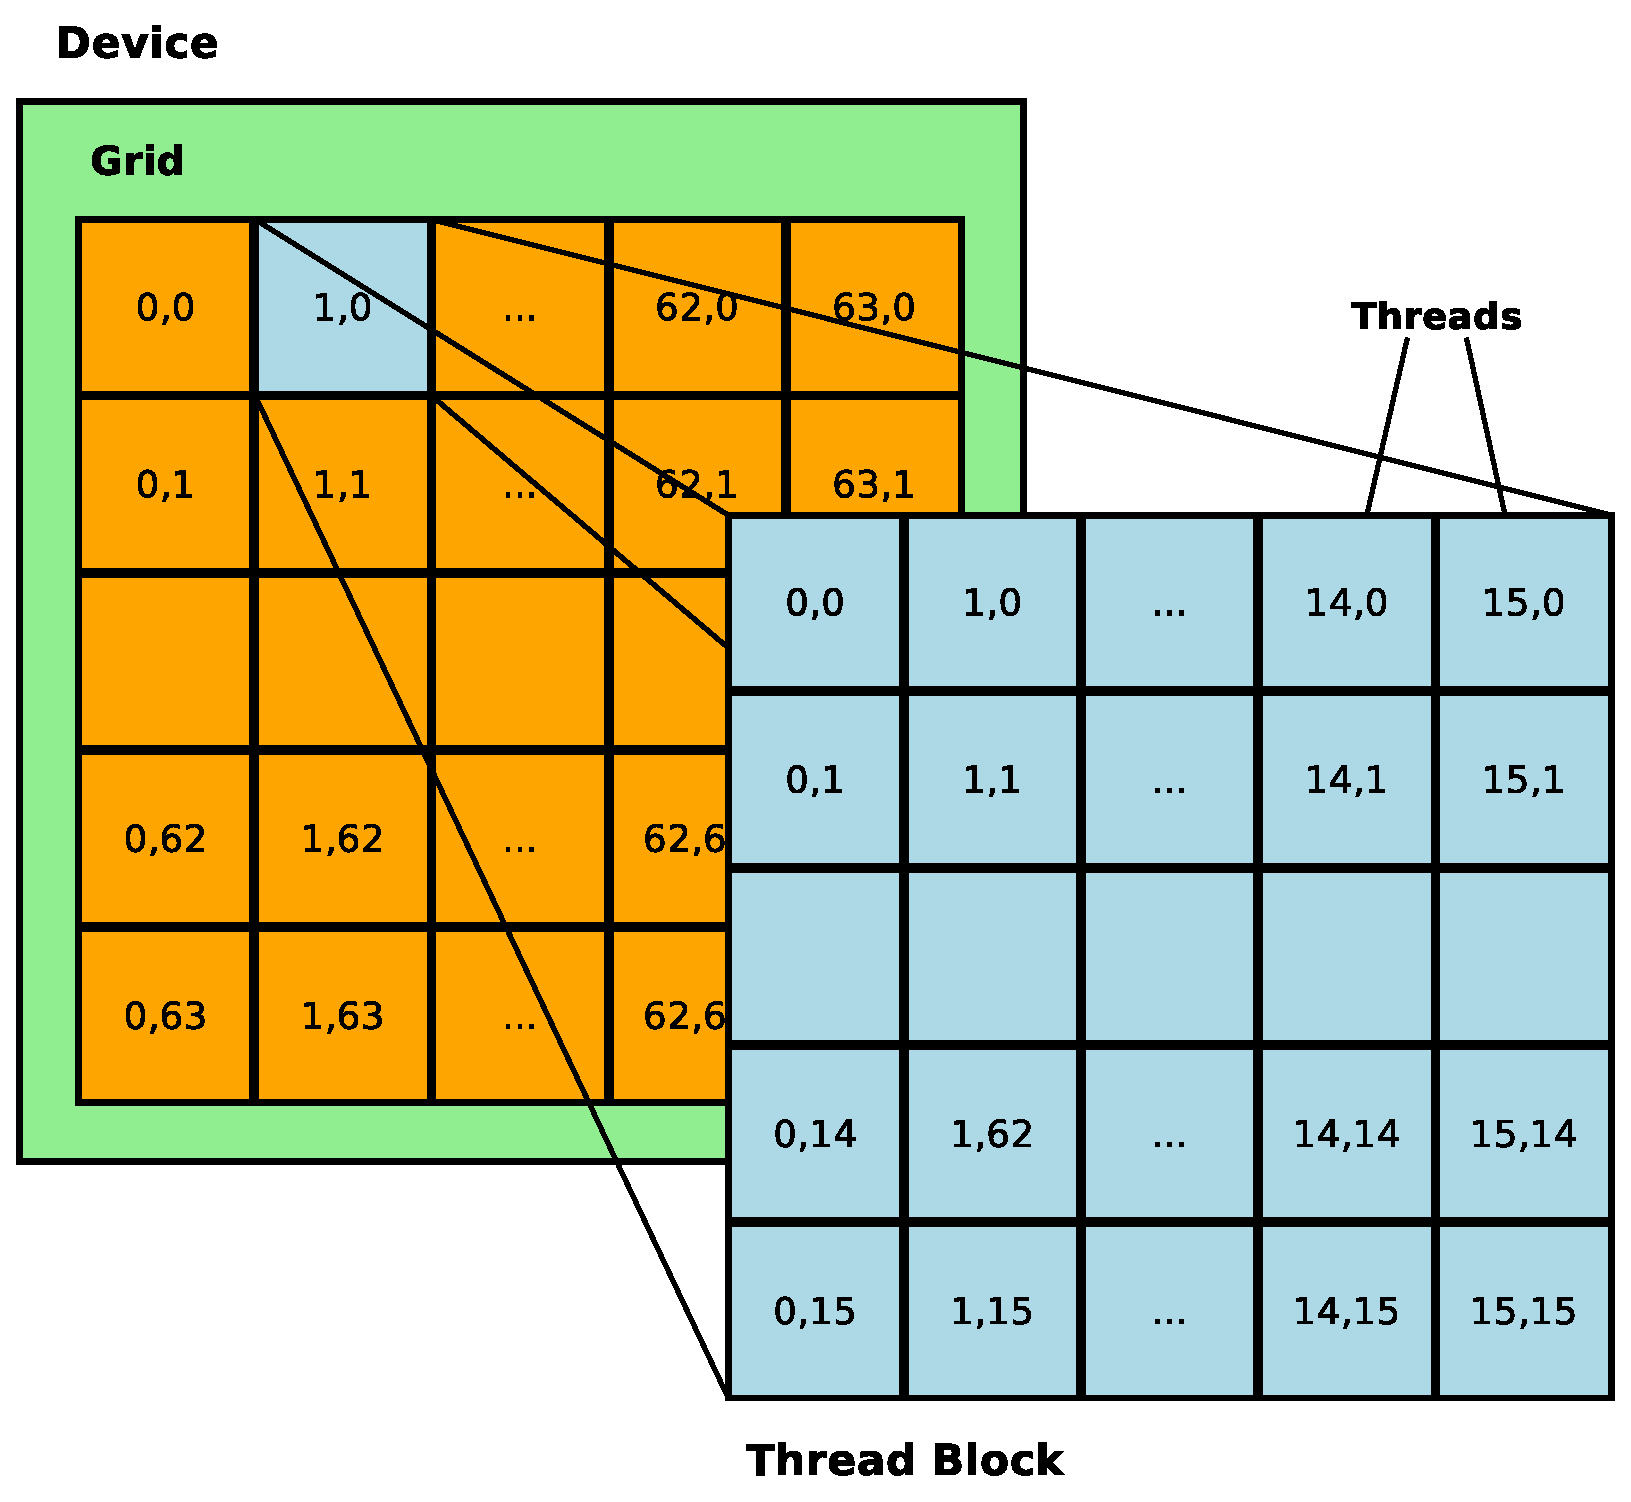
\includegraphics[width=0.9\textwidth]{grid}
\caption{Execution model: A piece of data is called {\it work-item} (thread); a kernel has many work-items subdivided into many {\it work-groups} (thread blocks); each work-group process many work-items.}
\label{figure:grid}
\end{figure*}


%%%%%%%%%%%%%%%%%%%%%%%%%%%%%%%%%%%%%%%%%%%%%%%%%%%%%%%%%%%%%%%%%%%%%%%%%%%%%%%
\subsection{Memory Model}
%%%%%%%%%%%%%%%%%%%%%%%%%%%%%%%%%%%%%%%%%%%%%%%%%%%%%%%%%%%%%%%%%%%%%%%%%%%%%%%

Programmers in general are used to read and write freely in any type of memory. Using the CPU we can read and write from registers, local memory (stack), global memory (heap) and disk. Accessing data for a GPU is more restricted.

Data storage and communication within a device and between devices, mainly CPU and GPU, is dictated by the memory model. It can represented in Figure \ref{figure:memory}. Again, every vendor use the same four memory types but with a different name. This is true for DirectCompute, CUDA and OpenCL.

\begin{figure*}[!ht]
\centering
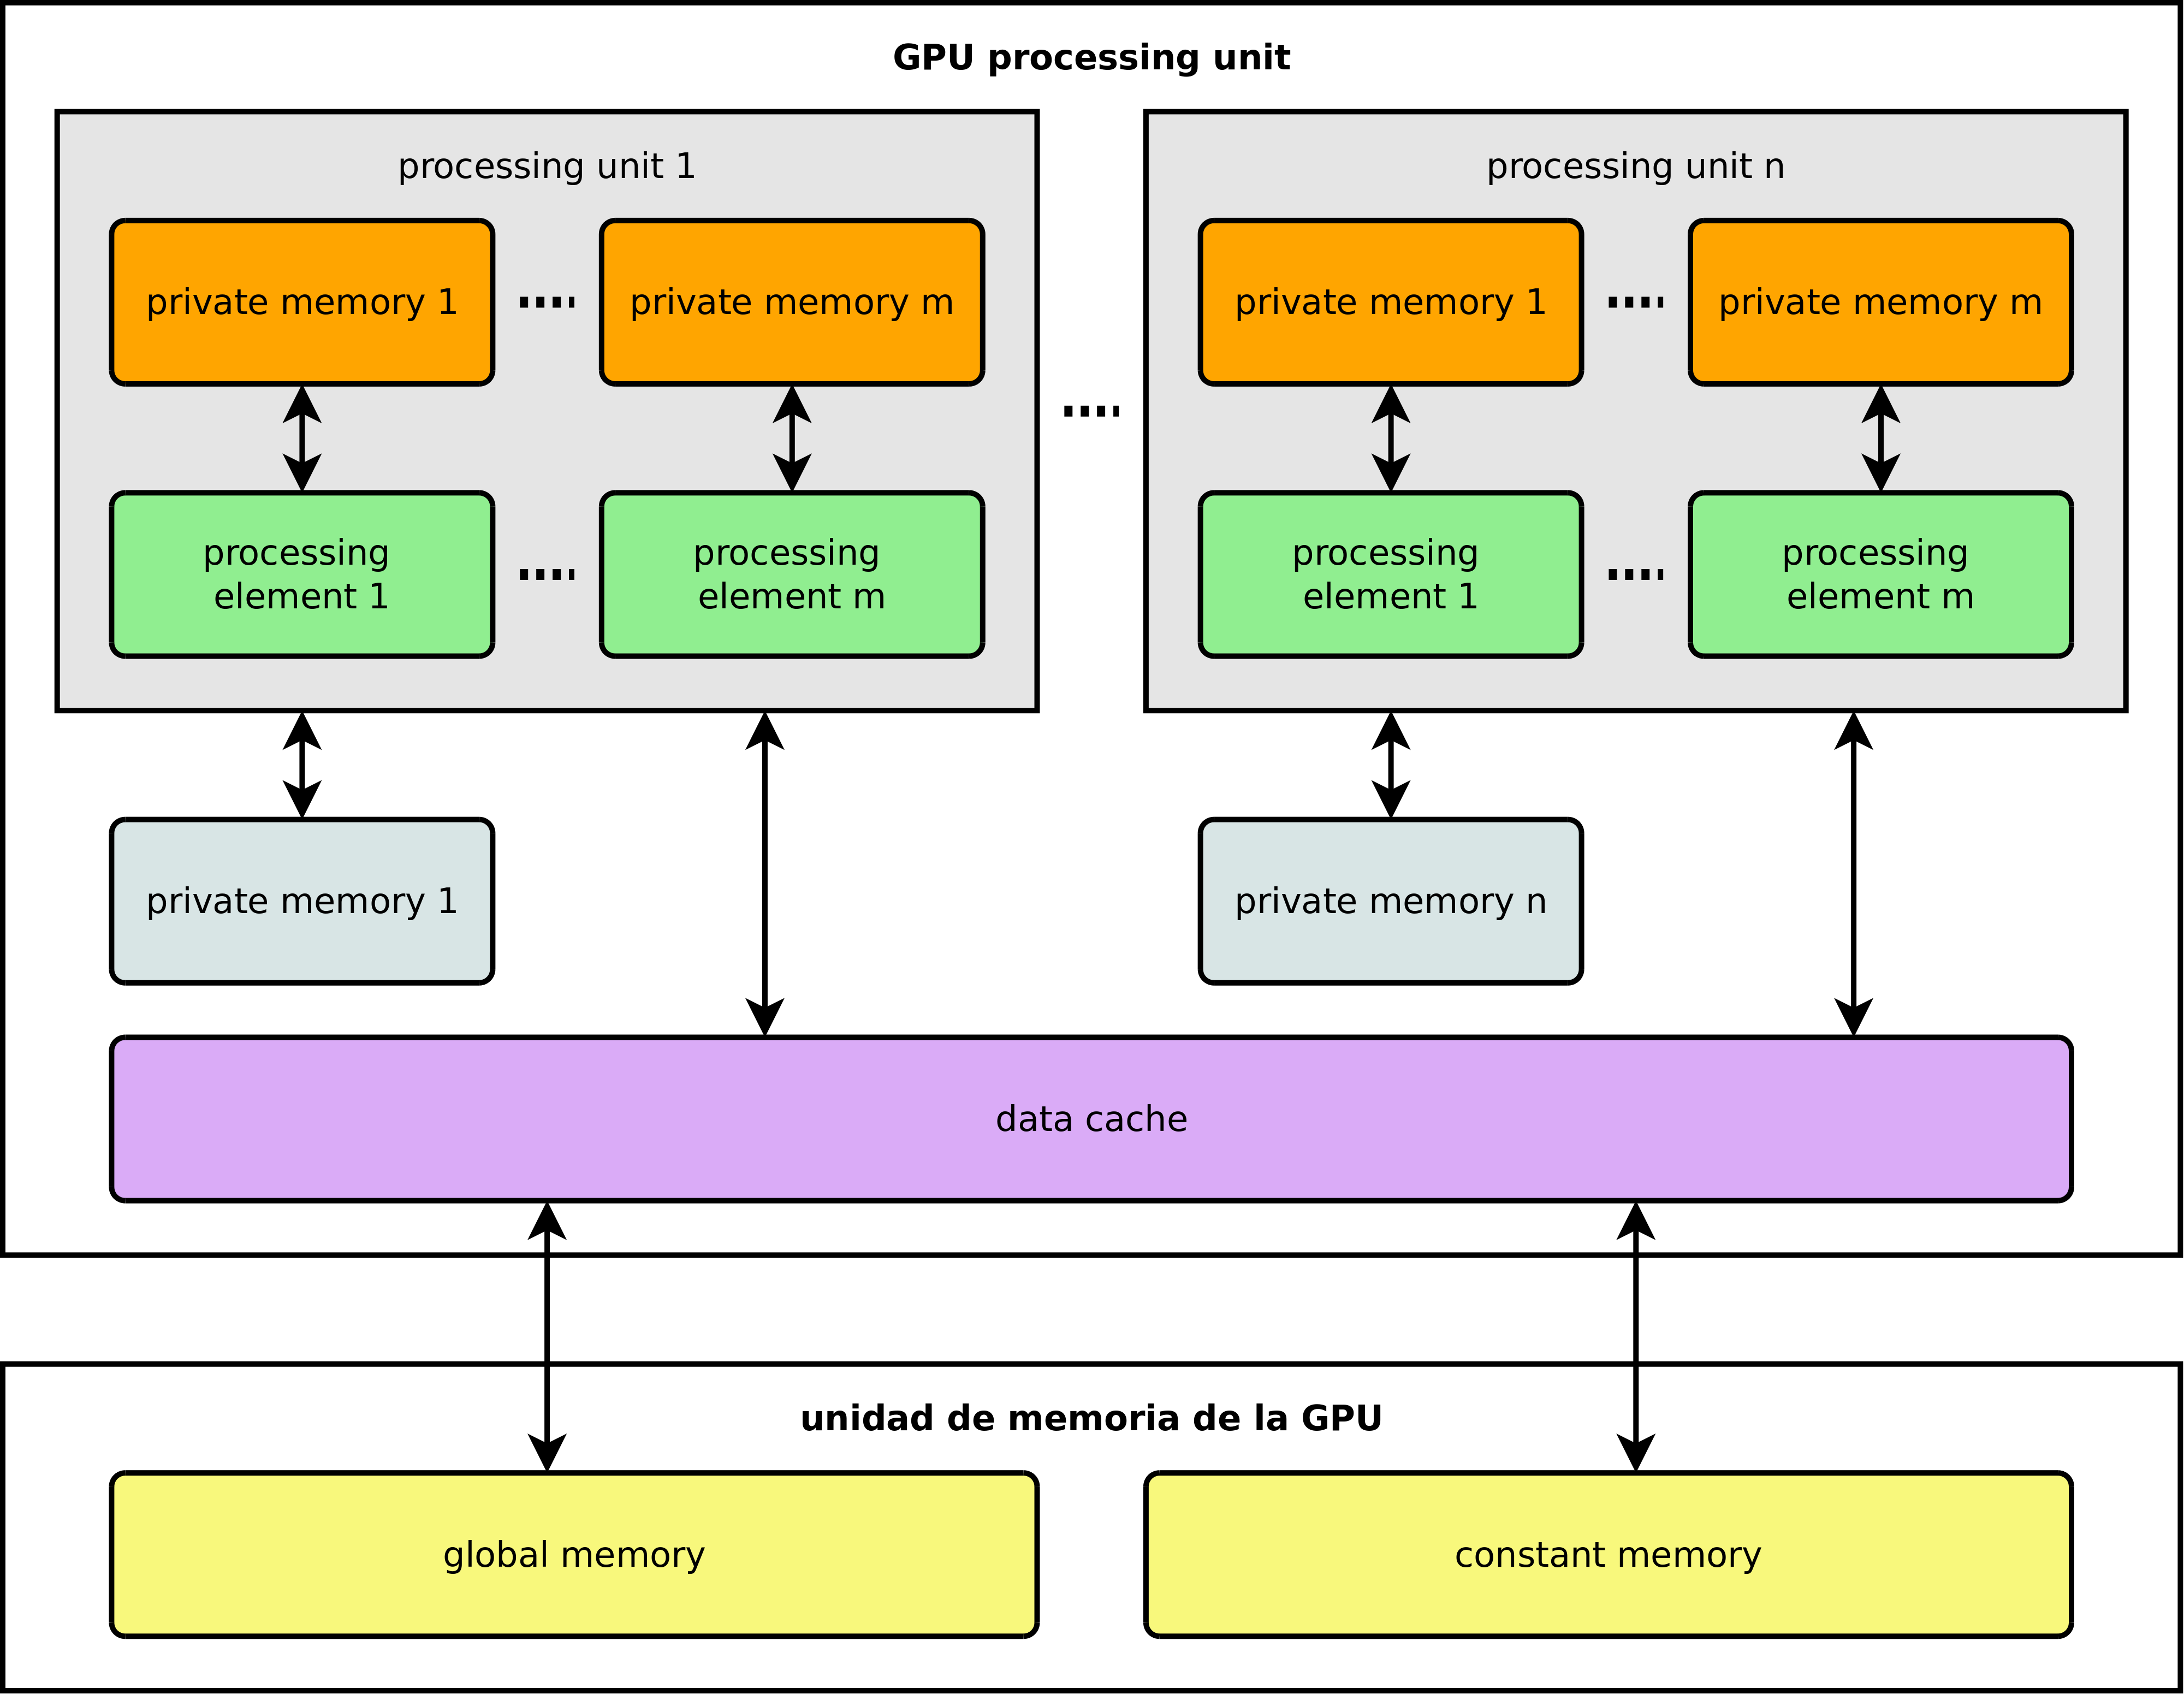
\includegraphics[width=0.9\textwidth]{memory}
\caption{The memory model defines how data is stored and moved between CPU and GPU. Global memory is RW for both CPU and work-items; constant memory is RW for CPU and RO for work-items; private memory is RW for a single work-item; local memory is RW for a work-group.}
\label{figure:memory}
\end{figure*}

\begin{itemize}
\item Global memory: any work-item and the host CPU can read and write.
\item Constant memory: any work-item and the host CPU can read this read-only region. Writing is only allowed to the CPU.
\item Private memory: a single work-item can read and write from it and is inaccessible for the host CPU. Most computation should be done here because it is the fastest one and the the most critical in terms of performance.
\item Local memory: a single work-group can read and write on it and is inaccessible for the CPU. Its main target is to share data between a limited number of work-items.
\end{itemize}

The need to move data in and out of the GPU memory is very common; it
will happen when a calculation is started or when results are
gathered. If the bandwidth consumed by this process involves an
excessive amount of time the target speedup can be ruined. Data
movement should be avoided or at least minimized. This bandwidth
problem has arisen many times in the computation field.

Every time a new powerful device has appear we must feed it  data fast enough. Two solutions of recent appearance try to alleviate it. The first is a
fourth level of cache between the CPU and the GPU. %reference - JJ
This is only useful
when both processors are glued together in the same chip or
encapsulation. The second solution involves changing the way we access
memory from GPU and its called Heterogeneous System Architecture
(HSA). % reference - JJ
HSA shares data between CPU and GPU in a seamless way, avoiding
as many memory copies as caches permits. This way both devices can
share a common memory architecture.

% You always have to relate whatever you say with the paper objectives
% - JJ

%%%%%%%%%%%%%%%%%%%%%%%%%%%%%%%%%%%%%%%%%%%%%%%%%%%%%%%%%%%%%%%%%%%%%%%%%%%%%%%
\section{Parallelizing EAs on GPGPUs}
\label{sec:parallelizing}
%%%%%%%%%%%%%%%%%%%%%%%%%%%%%%%%%%%%%%%%%%%%%%%%%%%%%%%%%%%%%%%%%%%%%%%%%%%%%%%

This section describes the most important frameworks used to
parallelize EAs to take advantage of the power of GPGPUs. In addition,
common issues and constraints to take into account when such a
parallel evolutionary approach is going to be implemented are also
pointed out.

%----------------------------------------------------------------------
\subsection{Frameworks to parallelize EAs on GPGPUs}

Since the creation of the EAs, many Universities and research groups have developed a number of frameworks to facilitate the implementation of this kind of algorithms. Many of them include implementations for the most common operators, problems and individual representations, using different technologies and programming languages.

The most complete and comprehensive review of these kind of frameworks was proposed by Parejo et al. \cite{springerlink:10.1007/s00500-011-0754-8}. It is a comparative study of metaheuristic optimization frameworks, and therefore it is not focused only on EAs. The criteria for comparison is a set of 271 features grouped in 30 characteristics and 6 areas. These features include the different metaheuristic techniques covered, mechanisms for solution encoding, constraint handling, neighborhood specification, hybridization, parallel and distributed computation, software engineering best practices, documentation, and user interface. However, none of the ten most extended optimization frameworks, ECJ, ParadisEO, Eva2, FOM, jCLEC, OAT, Opt4j, EasyLocal, HeuristicLab and MALLBA, included references to GPU capabilities when this paper was published.

However, a few years ago, some of these EA-based frameworks have added some
kind of GPU integration. Several authors have created library
extensions to the frameworks, in order to allow the evaluation of the
individuals in GPGPUs (which is normally the hardest computational
part). For example, Robilliard et al. \cite{RobilliardECJGPU08} did it
for ECJ, and Cano et al. for jCLEC
\cite{SpeedingTheEvaluationofGPCano:2012}.
On the other hand, ParadiseEO-MO-GPU \cite{MealbParadiseoGPU13}, another framework built upon an existing one, for now is only focused in single solution metaheuristics, and it does not support population-based ones, such as EAs.


PUGACE \cite{5586286} is one of the few new frameworks focused exclusively on the execution of EAs in GPGPUs. It is based on MALLBA and uses CUDA to execute cellular GAs (cGAs), but only for linear neighborhood structures. %The architecture of this framework is presented and experiments with the QAP problem are performed. Fitness evaluation uses a thread for each chromosome. Speedups for several problem instances varies from $\times15$ to $\times18$. The execution platform was a Pentium Dual Core at 2.5Ghz and an nVidia GeForce 98000 GTX+.

Finally, EASEA \cite{Maitre:2009:CGP:1569901.1570089} attempts to facilitate the development of EAs to be run in GPGPUs by compiling the code from a specific algorithm specification language (EASEA) into code suitable to be run in a CPU-GPU manner.
However, as in previous frameworks, only the code for the fitness
evaluation is sent to the GPU to be run in parallel, so the parallelization just affects to a part of the algorithm.
% That is not good because... JJ
% Antonio - written

%----------------------------------------------------------------------
\subsection{Requirements and constraints to parallelize EAs on GPGPUs}

The first step for parallelizing an evolutionary algorithm using a GPGPU is to study the GPU architecture, as the cards of different families would have special features which the programmer has to consider, in order to really take advantage of the hardware.
Thus, the algorithm and so its source code must be adapted to the GPU architecture in which the algorithm will run.
This task should be conducted carefully, since a code that has not been properly adapted might expend a higher time to run than its sequential version.

Next, usual basic steps a researcher (programmer) should consider in order to conduct a standard - and very common - parallelization of an EA on a GPU-based system are detailed.

The most extended parallelization approach is based on running the evolutionary loop on the CPU, while the GPU processors just run the evaluation stage (as this is usually the computationally hardest task). This approach is the simplest one, and the programmer only have to change a very specific part of the EA implementation. In this case, the EA is executed in two scopes, and some issues must be considered in each of them:

\begin{itemize}
\item In GPU scope:
	\begin{itemize}
		\item Allocate memory for the individuals to evaluate.
		\item Allocate memory for the data the individuals need for their evaluation (e.g. the matrix distances for a Travelling Salesman Problem).
		\item Allocate memory for the evaluation results.
		\item Each GPU processor evaluates one individual (or a part of it) using a kernel function. But while the first one is called/launched from the CPU scope, the rest of them might be called from the same scope or from the GPU one.
	\end{itemize}
\item In CPU scope:
	\begin{itemize}
		\item Copy the individuals and data for the evaluation from CPU scope to GPU scope.
		\item Copy the obtained results from GPU scope to CPU scope.
		\item Define the grid of threads for kernel function execution. Set the dimensions of each thread's block, determine how many blocks will be used, and how these blocks will be organized for the grid to use one, two or three dimensions.
		\item Call the kernel function or several functions using the grid of threads defined in previous step.
		\item Integrate the evaluation results with the rest of the evolutionary process.
	\end{itemize}
\end{itemize}

Previous steps can be implemented in any CUDA version. Moreover, in
recent versions of this programming language those steps can be
simplified, as the GPU processors are able to access CPU memory scope
directly.
However, this approach is not useful in most of the cases, since the
time required for CPU memory access is too large. Thus, normally, it
is only used when the data to access is just needed once for every
operation. If the evaluation process needs to use the data several
times, it might be better copying them to the GPU memory, in order to
speedup the next data loading.

There are other parallelization approaches where the GPGPU runs not
only the evaluation phase, but all the stages of the algorithm.
In the most usual implementation of this alternative, each thread or each block of threads must evolve a small number of individuals, so all the thread blocks must cooperate to evolve the whole population.
This approach can be easily implemented if the evolutionary algorithm is a fine-grained one.
In that case, the implementation will be based on assigning one
individual (or even a part of it) to each thread of a block. Then,
related threads must interact with their neighbors in order to
`co-evolve' individuals and also to carry out the rest of algorithm
stages.

Finally, it is very important to understand and to properly implement
the Single Program Multiple Data (SPMD)\cite{SPMD-wikipedia} programming
concept, in order to take advantage of it in the EA implementation. The programmer should always take into account the constraints related to the problem size, to the GPU, and computer, memory consumption, or to the synchronization of threads, as all these issues might affect the obtained performance.
% The different papers should have been here, or at least some
% introduction - JJ


%%%%%%%%%%%%%%%%%%%%%%%%%%%%%%%%%%%%%%%%%%%%%%%%%%%%%%%%%%%%%%%%%%%%%%%%%%%%%%%
\section{Parallelization Taxonomy}
\label{sec:taxonomy}
%%%%%%%%%%%%%%%%%%%%%%%%%%%%%%%%%%%%%%%%%%%%%%%%%%%%%%%%%%%%%%%%%%%%%%%%%%%%%%%

% This is a repetition of subsec:eas-distributed:parallel . Why don't
% you put them together? - JJ
% Antonio - It is not the same as in that section. That was an introduction and this is a (similar) taxonomy. I have clarified this inthe text and removed those redundant paragraphs/sentences.
In this section, a taxonomy to distinguish between the different
distribution methods applied in the literature is proposed.
It is inspired by the classical models used in the distribution of EAs, described in Section \ref{subsec:eas-distributed:parallel}.
%As stated before, even if there are many different bioinspired approaches included in the bibliography, we are mainly focused in this work on Parallel Evolutionary Computation (EC).
%That is the most extended metaheuristic to address many types of large or complex problems, which require some kind of parallelization to be solved with enough quality and on a reasonable quantity of time.

We take as a reference the survey by Alba \cite{Alba2005book}, who reviewed many parallel metaheuristics on EC. Most paradigms were identified with respect to
parallel/distributed EAs, according to Flynn's taxonomy, under the
Multiple Instruction Multiple Data (MIMD) category. This argument has
been fairly valid during the last two decades because the most
dominant platform for running parallel/distributed EAs were
distributed memory architectures, like clusters. However fine-grained
EAs deployed on massive parallel processors (MPPs) are resurfacing,
due to GPUs architecture gives low cost support for them.

The parallel EAs community has a big amount of contributions using
% wide legacy is not a thing - JJ
% Antonio - fixed
MIMD architectures, but a very little regarding SIMD systems, probably due to the MIMD dominance over SIMD.

Nevertheless, when the research community uses GPGPUs, all the EC approaches are parallel, so we have revised the bibliography taking in mind how an algorithm has been parallelized using that paradigm. Thus, for this survey, the specific metaheuristic used in every paper is being placed in a secondary position.
For that reason, we focus the rest of the survey on the different ways for implementing Parallel Evolutionary Algorithms (PEAs) as Zhang and Zhenming proposed in \cite{ZhangImplementationserverClient}: master-slave model \cite{man-leung-wong-parallel-2005}, fine-grained model \cite{jian_ming_li_efficient_2007}, coarse-grained model \cite{Maitre:2009:CGP:1569901.1570089}, %\cite{pospichalParallelGeneticAlgorithOnCUDA2010}
or hierarchical models  \cite{DBLP:conf/gecco/PospichalMOSJ11},  which use two or more of the previous parallel approaches in an hierarchical way.


%%%%%%%%%%%%%%%%%%%%%%%%%%%%%%%%%%%%%%%%%%%%%%%%%%%%%%%%%%%%%%%%%%%%%%%%%%%%%%%
%\subsection{Taxonomy} % A section named taxonomy can't have a
                      % subsection called taxonomy. Simply eliminate
                      % the subsection, and leave this as an
                      % introduction - JJ
% Antonio - you're right
%%%%%%%%%%%%%%%%%%%%%%%%%%%%%%%%%%%%%%%%%%%%%%%%%%%%%%%%%%%%%%%%%%%%%%%%%%%%%%%

Thus, the proposed taxonomy is based on the classical approach followed by other authors, but it adds two new groups that we consider important: the hierarchical and the non-standard models.

% -----------------------------------------------
\subsection{Master-slave approaches}
\label{subsec:serverClientapproaches}
Master-slave Evolutionary Algorithms traditionally solve problems
involving computationally expensive fitness functions, where the
master node runs the entire algorithm while the slaves execute the
fitness evaluation of the individuals. Using this approach, the
evaluation of the fitness function is not sequential, but in parallel,
so the master-slave version is more efficient because the evaluations
usually are the more expensive portion of the total run time.
% if this is a different classification, this should go with the
% section mentionad above. just say that they are classification along
% different axes, but there are too many classifications for a single
% paper - JJ
% Antonio- the classification is similar, but here we focus on the existing approaches in the GPGPU literature ad we extend the explanation given in previous section

% -----------------------------------------------
\subsection{Fine-grained approaches}
\label{subsec:finegrainedapproaches}

Cellular Evolutionary Algorithms (CEAs) or Fine-grained Evolutionary
Algorithms have not had as much impact as other types of PEAs. The
main reason is that they adapt themselves very well to the special
hardware architecture, with shared memory, but very badly to other
distributed memory architectures. On the other hand, parallel
distributed memory architectures supply all loosely coupled algorithms
and the fine-grained EAs are not included into this category. The main
reason behind that is the high cost of building massively parallel
architectures which normally attracted fewer researchers to work on
fine-grained EAs. However, a review of the trends in parallel
architectures foresees a strong increase in fine-grained EAs face to
face other EA categories. This is due to three reasons:

\begin{itemize}
\item Growing trend of massive number of processors on chip or card.
\item The high inter-processors speed which is a major factor affecting the efficiency of fine-grained EAs.
\item The huge low cost of these architectures which attract a wide base of researchers and developers.
\end{itemize}

For this category of algorithms, each individual is a parent at the beginning of the algorithm and it looks for the second parent by selection in a neighborhood. As a result CEAs provide automatic niching effect, avoiding an early convergence.

% -----------------------------------------------
\subsection{Coarse-grained approaches}
\label{subsec:coarsegrainedapproaches}

These approaches work with a set of sub-populations, normally a part
of the whole population, distributed in different nodes, being every
node devoted to work with just one of them, so they can work in
parallel independently. Each of these sub-populations is known as an
`island'. In the standard model, after a number of generations one or
more individuals, normally the best, are interchanged, as dictated by
migration rate, between islands, which are connected following a
specific neighborhood topology.


% -----------------------------------------------
\subsection{Hierarchical approaches}
\label{subsec:hierarchicalapproaches}

This hybrid model just utilizes two or more of the master-slave, coarse-grained and fine-grained approaches in an hierarchical method. At the higher level, an island model algorithm runs while at the lower level, the demes, or sub-populations, are running in parallel, fine-grained, master-slave or even another island model with high migration rates. Hybrid models are not the most common in traditional implementation of EAs due to:
\begin{itemize}
 \item The need for additional parameters related to the more complex topology structure.
 \item The need for `quite rare' hierarchical parallel architectures to host hybrid algorithms.
\item The high complexity of programming such models.
\end{itemize}

Nevertheless, for the GPUs, hybrid EAs are a perfect candidate to exploit the hierarchical memory and flexible block sizing, by means of well structured populations.


% -----------------------------------------------
\subsection{Non-standard approaches}
\label{subsec:nonstandardapproaches}

By the end of the work we have included a subsection for non-standard
approaches \cite{DBLP:conf/gecco/PospichalMOSJ11} including papers
which may not be included in any of the previous ones because they
mapped the algorithms and the problem they solve in a special way that
cannot be considered as fine-grained, coarse-grained or master-slave
ones.



%%%%%%%%%%%%%%%%%%%%%%%%%%%%%%%%%%%%%%%%%%%%%%%%%%%%%%%%%%%%%%%%%%%%%%%%%%%%%%%
\section{Literature analysis and review}
\label{sec:survey}
%%%%%%%%%%%%%%%%%%%%%%%%%%%%%%%%%%%%%%%%%%%%%%%%%%%%%%%%%%%%%%%%%%%%%%%%%%%%%%%

In this section we present a quantitative analysis of published papers
on EAs on GPUs. Then, the most relevant ones are classified following
the previously described taxonomy.

Firstly, an in-depth analysis of the existing related literature has been done. In order to conduct this analysis we performed the query ``\textit{(GPGPU OR GPU) AND (GENETIC OR EVOLUTIONARY)}'' in the Web Of Science (WoS) \cite{wos} database, referred to any part of the publications, and just enclosed into {\em Computer Science} research area.
% Antonio - comprobar si se buscó en cualquier parte de los artículos
% Check out these comments - JJ
It yielded 329 references, from which we eliminated those references unrelated to the scope of this paper (for example, those whose topic is related with genetic engineering and not with genetic algorithms). After that removal, 194 results remained, which were carefully read in order to extract its features and useful information for this survey.
% maybe we should rewrite these sentences avoiding the  "we"  [pedro]
% Antonio - I have rewritten this in par i order to avoid somany 'we's

Looking at the publication rate per year inside this scope, it can be noticed in Figure \ref{figure:publications}, that the publication figures has been increased every year, starting from 2004, being nowadays a very appealing and prolific field for researchers  (according to the results).

\begin{figure*}[!ht]
\centering
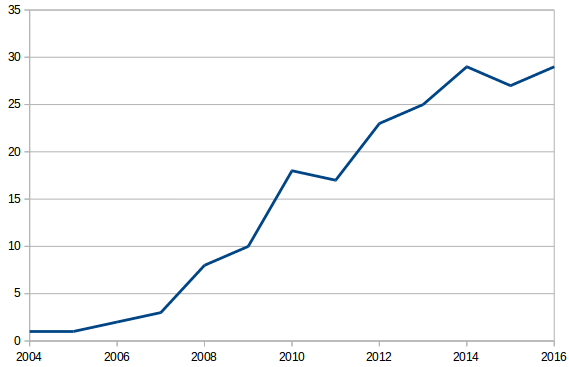
\includegraphics[width=0.75\textwidth]{years}
\caption{Papers published per year in the scope of EAs on GPGPUs, according to Web of Science database.}
\label{figure:publications}
\end{figure*}


Regarding the type of EA implemented or studied in those papers, Figure \ref{figure:type_algorithm} shows the percentages of the different approaches. The most prolific ones are GAs, since it is the classic optimization method inside EAs. It is easy to implement and usually yields very good results.  GP and DE are more specific and thus, less extended or used. `Others' refers to EAs such as EDA (Estimation of Distribution Algorithm), SGS (Systolic Genetic Search) or MA (Memetic Algorithms), to cite a few.

\begin{figure*}[!ht]
\centering
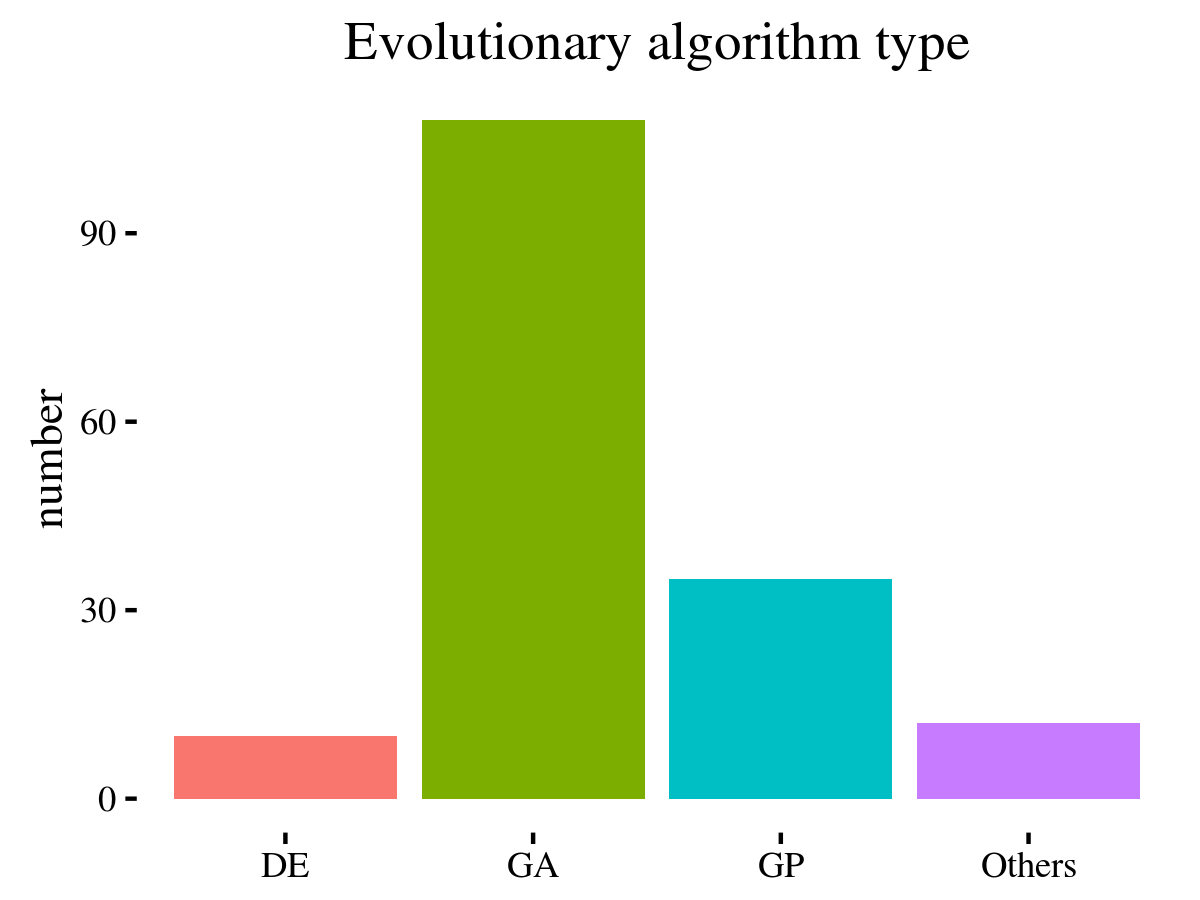
\includegraphics[clip,width=0.9\textwidth]{algorithmtype}
\caption{Type of Evolutionary Algorithm implemented in the analyzed publications.}
\label{figure:type_algorithm}
\end{figure*}

Finally, the majority of the analysed publications deal with solving real problems as  presented in Figure \ref{figure:type_problem}. This means that parallelization by means of GPUs is very effective and can be used in relevant and very hard problems, as real world ones frequently are.

\begin{figure*}[!ht]
\centering
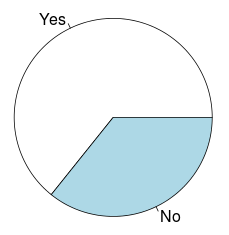
\includegraphics[clip,width=0.9\textwidth]{realproblem}
\caption{Portion of the analyzed publications which address real problems.}
\label{figure:type_problem}
\end{figure*}


Once analyzed the whole literature from a general perspective, the following sections will go through each of the different groups of the proposed taxonomy. Then, each of the most representative or relevant works (mainly according to their number of citations) are reviewed and commented.

%After reading this section it is clear than PEAs is an active research field and there are so many different variations that almost for sure one of then can fit the needs of most users. Following this reasoning, in the next 5 sections, the most representative works of every type of EA are going to be presented for your convenience.

%%%%%%%%%%%%%%%%%%%%%%%%%%%%%%%%%%%%%%%%%%%%%%%%%%%%%%%%%%%%%%%%%%%%%%%%%%%%%%%
\subsection{Server-client approaches}
\label{sec:serverClient}
%%%%%%%%%%%%%%%%%%%%%%%%%%%%%%%%%%%%%%%%%%%%%%%%%%%%%%%%%%%%%%%%%%%%%%%%%%%%%%%

As a GPGPU implementation, the GPU is responsible for fitness
evaluation but it does not get involved with other phases of the
algorithm such as crossover, selection or even population ranking for
the next generation. In this approach, every generation the
individuals are copied to the global memory of the GPU, so every
single processor gets one or more individuals from global memory and
puts them into the shared memory, in order to decrease global memory
overhead. After that, each thread evaluates it or them, and stores the
result into the global memory again. Usually each single core
evaluates one individual. The programmer has to minimize the number of
global memory accesses, as well as to minimize data transfers between
CPU and GPU. Some additional problems might be faced, like for
example, individuals that require additional data for being evaluated,
such as a distance matrix or a data set. This additional information
might be copied from CPU to GPU once at the beginning of the process,
so the threads might access this data for evaluation minimizing CPU/GPU
traffic.

One of the first proposals for parallel Evolutionary Computation using
a GPU was done by Wong et
al. \cite{man-leung-wong-parallel-2005}. They presented an
Evolutionary Programming (EP) algorithm
% without crossover EP does not have crossover - JJ
% EP is not included in the list of algorithms - JJ
for solving five simple test functions, called Fast Evolutionary Programming
(FEP). In this master-slave approach, some actions such as the main loop of the algorithm were executed in the CPU, while evaluation and mutation were run within the GPU device because both steps do not need of external information exchange. In this case, the reproduction process implies interaction among, at least, two individuals so the authors eliminated this step in the algorithm. A maximum speedup of $\times5.02$ was obtained when the population size increases. This is the most common organization in GPU implementations, since no
interaction among individuals is required during the evaluation, so
this process can be fully parallelized. In that paper the individuals
was real-coded and the genomes were mapped into the texture
memory. Each GPU thread evaluated one individual and returned its
fitness at the end of the parallel process to the CPU, for the next
evolution cycle.

A Genetic Programming (GP) method proposed by Harding and Banzhaf \cite{4215552} is another example of execution of the EA using the GPU for fitness evaluation, while the rest of the steps are executed on the CPU. In this paper real-coded expressions were tested in up to 10000 nodes, boolean expressions in up to 1500 nodes, and some expressions of real world problems in up to 10000 nodes. Results yielded a speedup of thousand times in some instances.
Besides, Chitty et al. \cite{Chitty2016} proposed different techniques to improve the performance of a graphics card implementation of tree-based GP in order to better exploiting this faster device. Authors demonstrated that both L1 cache and shared memory need to be considered for obtaining the maximum performance.

Hierarchical parallel GAs have been adapted using other models. For example, Zhang et al. \cite{ZhangImplementationserverClient}, proposed the use of {\em deme} model at high level, and a master-slave schema at low level. In this case, the CPU initializes the population and distributes the individuals to thread blocks in shared memory. Then, the GPU threads within each block run a GA independently, by applying selection, crossover, mutation and performing the evaluation; and it migrates individuals to other thread blocks in its neighborhood. However, no speedup results were reported in this paper.

Van Luong et al. \cite{5586403} published in 2010 a methodology for mapping the search space onto the GPU memory hierarchy in three levels: (1) the distribution of the search process among the CPU and GPU, (2) the mapping of the neighborhood in the GPU threads, and (3) the effective usage of the texture memory in the context of hybrid EAs. Experiments to solve the QAP problem with CUDA were presented, where the evolutionary process was performed in the CPU and the generation of the Local Search neighborhood were conducted on parallel in the GPU, achieving an acceleration of $\times14.6$ times faster. Hardware used was Core 2 Duo 2.67GHz and Nvidia GTX 280. This work also showed the benefits of using a conjunction of CPU + GPU, being the GPU used only for intensive calculations.

%There are other papers related with the previous approach, like the one by Tsutsui et al. \cite{Tsutsui:2011:GECCO}. This work uses a master-slave approach with an Ant Colony Optimization (ACO) algorithm \cite{Dorigo:1999:ACO:329055.329062} and Tabu Search \cite{Glover:1997:TS:549765}. Tsutsui uses an Intel Core i7 965 (3.2 GHz) processor and a single NVIDIA GeForce GTX480 GPU. They compare CPU and GPU implementations with and the results showed that GPU computation with MATA, an efficient method for thread assignment cost which they call Move-Cost Adjusted Thread Assignment, showed a promising speedup compared to computation with CPU. PABLO: REMOVED THIS, IT IS AN ACO

There are papers related with other subjects % cuales subjects? - JJ
like \cite{Pedemonte:2011:BOG:2001858.2002031} which studies the impact of using different representations for binary problems in GPUs to evaluate GAs: boolean data type versus packing multiple bits in a non-boolean data type. The execution platform was a PC with a Quad Core Intel Xeon E5530 processor at 2.4GHz and a Tesla C1060 with 240 CUDA cores. The CPU only calculates the initial population and a matrix of random numbers to be used in crossover and mutation by the GPU. The authors reviewed the problem of the data types when GPGPU is used. Several data types of 8, 16, 32, and 64 bits are compared in CPU and GPU versions. Results showed that packing in 32 bits data types achieve speedup values of up to $\times100$ compared with boolean data types, specially when the size
of the instances increases. This make sense because the Tesla C1060
are equipped with 32-bit integer ALUs.

Cano et al. \cite{SpeedingTheEvaluationofGPCano:2012} described a massively parallel evaluation model using a Genetic Programming algorithm for evolving rules for dataset classification. They copied the dataset to the GPU global memory, and evaluated the rules (individuals) for each instance of the dataset in parallel (match kernel). At the end, each successful match was reduced getting each individual fitness (reduction kernel). The implementation, based on CUDA, speedups the fitness calculation phase and greatly reduce the computation time. Results were compared using one, two and four CPU threads and the combination of one or two GPUs of different features (285 cores for GPUa -NVIDIA GeForce 285 GTX- or 480 cores for GPUb -NVIDIA GeForce 480 GTX-). They test three classification algorithms and the results were not very significant for small datasets, but they increased the speedup with large datasets until $\times820$ using two GPUs with 480 cores each one.

The work by Chitty \cite{Chitty16FastParallel} uses a Master-Slave architecture for evaluating at time the population for four GP problems. The results were achieved using an NVidia GeForce Kepler 670 GTX graphics card and compared with a previous one-dimensional stack approach for the same problems. The author fit the algorithm until to observe a peak computational speed of over 55 billion Genetic Programming Operations per second a twofold improvement over the previous one-dimensional stack approach.


Recent works are currently being applied to real-world problems. Jaros et al. \cite{Jaros14Wormhole} use GPUs to lower the run time and improve the quality of the solutions in the problem of wormhole switching in collective communications. The start from an evolutionary tool capable of finding optimal communication schedules for various communication patterns on wide range of interconnection networks topologies of up to 256 nodes. The tool consumes tens of hours so they decide to improve it. As the fitness evaluation was responsible for the 93\% of the execution time this was the only part moved to the GPU. In a first step only one GPU was used with speedups up to $\times5$. After that they made a new implementation capable of using 8 GPUs and 30 times faster than the original.

In \cite{Contreras:2012:UGA:2150467.2150469} the authors use a CPU-GPU architecture for stock market trading. The proposed architecture offers the benefices of GPU distribution for stock market researchers, rather for computer architecture experts. The authors used Jacket \cite{jacket:Matlab}, a software platform for the rapid development of GPGPU computing applications within the MATLAB computing environment, C, and C++. However, this framework is no longer available \footnote{\url{http://blog.accelereyes.com/blog/2012/12/12/exciting-updates-from-accelereyes/}}. Steps and guidelines to migrate from CPU code to GPU code are explained, what is a great contribution, because usually, the authors do not include this information in the papers. The algorithm run in the CPU, but all  {\em for} loops in selection, evaluation, crossover and mutation are translated to Jacket's {\em gfor} to be parallelized in the GPU. Three different CPU configurations are used for the experiments: Pentium 4, Pentium SU41000 and Intel Core i7-860. The former is also combined with an nVidia 460GTX for GPU experiments. Different population size are also tested. The time is reduced to 65\% in comparison with the CPU version. Other conclusions are obtained: speedups with high number of individuals, rather than increasing the number of evaluations; and time reduction for  tournament selection  over roulette-wheel selection.

Stock market trading analysis has also been recently addressed by
using GP in GPUs. The algorithm described in the work by Sungjoo et
al. \cite{Sungjoo15fastknowledge} is used to solve the problem of
knowledge discovery in stock market time series, i.e. finding the
so-called precursor patterns, which model events occurred in the time
series. Thus, every individual (tree) in the GP algorithm is a
pattern, which must be matched against the whole dataset to find
out if it is a precursor. This is what the evaluation function
does. The time series is divided into different subsets, and stored in
several GPUs. The data is then copied once and just the new
individuals to evaluate and the partial results of the evaluation must
be transferred and updated, avoiding bandwidth problems.
The run is conducted for 50 generations and with 500 individuals of a maximum depth of 3 levels, using a i7-3820 CPU and 8 CUDA GPUs (GeForce GTX 690).
% You need to give that amount of details? - JJ
The authors considered
512 threads per block, 260 blocks per grid and just one grid per
GPU. The comparison in performance yields a reduction of 56 times for
just one GPU to 277 using all of them. This improvement is obtained using
local memory allocation, using the shared memory of blocks instead
yields a smaller improvement of around 188 times faster in the best
case. Regarding the influence of individuals' tree size (number of
nodes) in the performance, the authors show that the running time
grows for just one GPU, but when more than four are used, this growing
is minimum and could be assumed in order to improve the quality of the
results. % Some comment with respect to bandwidth? - JJ


%%%%%%%%%%%%%%%%%%%%%%%%%%%%%%%%%%%%%%%%%%%%%%%%%%%%%%%%%%%%%%%%%%%%%%%%%%%%%%%
\subsection{Fine-grained Approaches}
%%%%%%%%%%%%%%%%%%%%%%%%%%%%%%%%%%%%%%%%%%%%%%%%%%%%%%%%%%%%%%%%%%%%%%%%%%%%%%%

Researchers implement fine-grained algorithms using GPGPU, making
every scalar processor (SP) to evolve an individual. This individual
interacts with other SPs that belongs to the same Streaming
Multiprocessor (SM) to perform the basic operations of the algorithm
like crossover or mutation. In this approach a big part of the
algorithm runs within the GPU and not only the evaluation phase like
in previous section (\ref{sec:serverClient}). The GPU architecture
assists the neighborhoods emerge since each group of SMs have a shared
memory, where SPs access without penalty. The exchange of information
between individuals through this shared memory is
inexpensive. However, programmers have to be careful with the
information exchange between individuals in different SMs.

The second problem of this approach is the random number
generator. The CPU can easily generate random numbers, but the GPU is
not able to do this task.
% In fact, the CPU is not either. - JJ
% Antonio - fixed
So researchers have to think about how to solve this problem. Usually the algorithm's implementation generate at the beginning a big set of random numbers and they are copied to the GPU as a list. After that, the GPU uses the random list when needed and when it need. This approach saves time for random generation but the list of random numbers has to be limited. Moreover, all SPs could use the random numbers, so the list must be available for every
thread.


Yu et al. \cite{yu-parallel-2005} implemented the first real cellular EA using GPUs, for solving the Colville problem \cite{Ng:2005:DFF:1064290.1064296} in 2005. The population is distributed in a toroidal 2D grid and the classical Von Newmann neighborhood structure with five cells was used. Chromosomes and their fitness values were stored in the texture memory on the graphic card, and both, fitness evaluation and genetic operations, were implemented entirely with fragment programs executed in parallel on GPU. Real-coded individuals were represented as a set of 2D texture maps. BLX-$\alpha$ crossover and non-uniform mutation was developed as tiny programs on every pixel at each step in a SIMD-like fashion. They solved some optimization problems and reached a speedup of $\times15$ with a population of 512x512 individuals. They store a set of random numbers at the beginning of the evolution process to solve the random number generation problem when using GPU processors.

In 2006, \cite{man-leung-wong-parallel-2006} proposed a parallel hybrid GA (HGA) where the whole evolutionary process run on the GPU, and only the random number generation is done in CPU. Every individual is assigned to a GPU thread, and each one selects probabilistically an individual in its neighborhood to mate with it. Just one offspring individual is generated each time, and it replaces the old one in that GPU thread. The authors compare their implementation with a standard GA run in a CPU and the FEP \cite{man-leung-wong-parallel-2005} algorithm. Using a new pseudo-deterministic selection method, the amount of random numbers transferred from the CPU is reduced. HGA reaches speedup of $\times5.30$ when compared against the sequential version. In 2009 Wong et al. \cite{wong-implementation-2009} provide implementation details for fine-grained evolutionary algorithms.

Liu and Luo \cite{zhongwen-luo-cellular-2006} implemented a cellular algorithm on GPU to solve three different satisfiability problems (SAT)
using a greedy local search (GSAT) \cite{Selman93domain-independentextensions} and a cellular GA (cGA).
They saved local minimums using a random walk strategy, jumping to other search space location.
The cellular GA adopts a 2D toroidal grid, using the Moore neighborhood, stored on texture GPU memory. This implementation generates the random numbers in the GPU (using a generated seed on the CPU at the beginning of the process). They carried out the experiments using two GSAT implementations, CGSAT (with crossover and without mutation) and PGSAT (without crossover and with mutation) running them on CPU and GPU with different population sizes. A great time reduction was reached using the GPU parallelization approach (from 95ms to 18 ms for CGSAT and from 464ms to 77 ms for PGSAT).

Li et al. \cite{jian_ming_li_efficient_2007} proposed a cellular algorithm on GPU for solving some common approximation functions. The authors reported experiments using big populations (up to 10000 individuals) reaching speedups of $\times73.6$ for some implementations. The novelty of this paper is the bit dataset because it is not easy to deal with bit datasets using a GPU due to the memory size restrictions. The GPUs does not support binary operations, but in this paper the authors dealt with binary individuals of 24 bits  and simulated bit-operator by judging each bit of a binary value is 1 or 0. They faced a general problem for all GPGPU community with bit operations. They proposed to use random-textures for random numbers generation, but the random numbers were generated on CPU previously.

As in previous work, fitness evaluation and genetic operators were applied in the GPU by Gonz\'alez et al. \cite{springerlink:10.1007978-3-642-12538-619} by using CUDA, and storing individuals and their fitness values in the GPU global memory.
The difference is that they used a pseudo random number generator provided by the SDK of CUDA named Merseinne Twister. Some general discrete and continuous optimization problems were used in the experimental setup, and physical and numerical efficacy were compared with respect to CPU implementation.

In \cite{Li:2009:PIA:1726585.1726930} the authors proposed an Fine-grained parallel immune algorithm (FGIA) which is an Artificial Immune System combined with an EA. Three medium-size instances of the Travelling Salesman problem (TSP) were solved by using a fine-grained parallel algorithm with CUDA C. The algorithm enlarges the population size of FGIA maintaining better population diversity. As a remark, the authors included a sub-linear relation between the population size and the execution time, which made the proposal very useful for solving difficult problems that require huge population sizes.



Depending on the problem size, fine-grained approaches may improve the
efficiency with respect to the coarse-grained version. For example, in
the work of Franco et al. \cite{Franco15LargeScale}, two different
approaches for strategies for GPU implementations of the evaluation
stage of evolutionary rule learning are analyzed and the types of
problems where each method performs best have been identified. The
coarse-grained implementation is more conservative and only
parallelizes the evaluation of instances, while the fine-grained
implementation expands the parallelism to the attribute dimension and
is faster on data sets with 10 to 50 discrete attributes.


%%%%%%%%%%%%%%%%%%%%%%%%%%%%%%%%%%%%%%%%%%%%%%%%%%%%%%%%%%%%%%%%%%%%%%%%%%%%%%%
\subsection{Coarse-grained Approaches (Island Model)}
% why mix caps and not? - JJ
% Antonio - fixed
%%%%%%%%%%%%%%%%%%%%%%%%%%%%%%%%%%%%%%%%%%%%%%%%%%%%%%%%%%%%%%%%%%%%%%%%%%%%%%%

The coarse-grained algorithms are the most common among parallel EAs, as mentioned in Section \ref{subsec:coarsegrainedapproaches}, due to the inherent parallelization possibilities they offer. Thus, these algorithms require less tightly coupled parallel architectures, as compared to fine-grained ones.
This kind of EAs works by dividing the main population into sub-populations (also known as `islands') which evolve concurrently, and from time to time, some individuals are moved from one island to another (migration).
This basic feature of coarse-grained EAs hits a physical limit of
GPUs.

% a ver qué tal esta versión:     [pedro]
% Antonio - mejor. ;)
In order to run a coarse-grained EA using a GPU device, several kernels could be run simultaneously. In that case, each kernel could handle a sub-population of individuals, establishing some synchronisation points.
However, the GPU architecture is not designed for synchronising
different kernels into the same grid, which means that using a GPU to
run a coarse-grained EA might require changing some standard mechanisms
of the algorithm.


One of the first island models on GPU-based approaches was presented on the GECCO 2009 GPU Competition \cite{gecco2009CompetitionPospichal}. This technical report presented some technical details of an island model entirely hard-coded on GPU, with a ring-neighborhood topology. As it was a first attempt, the evolutionary operators implemented on GPU were only specific to the GECCO competition, and the validity of the experiments is not clear, since the approach just worked on a small number of problems.

However, after this, Pospichal et al. continued working on their approach \cite{pospichalParallelGeneticAlgorithOnCUDA2010,9253}. The authors mapped threads to individuals, and then, these threads-individuals could be synchronized easily in order to maintain data consistency. To decrease memory latency, the usage of an on-chip hardware scheduler was proposed, which swiftly swaps existing islands between multiprocessors, with the combination of a fast-shared memory. In this case, the population size was limited to 16KB per island (as on most GPUs at that time), so if the population was larger, the main memory would be used, implying a time increase. In fact, the inter-island communication was used, by relying on it the migration, based in an asynchronous unidirectional ring model. Even that, authors reported speedups up to $\times7000$ times higher on GPU compared to CPU sequential version of the algorithm.

Permutation domain problems have been studied by some authors. Tsutsui and Noriyuki \cite{1570355} also run a coarse-grained GA on a GPGPU, to solve the QAP problem using CUDA. Their model generated the initial population on CPU and copied it to the GPU VRAM; then, each sub-population in a GPU (NVIDIA GeForce GTX285) was evolved. At some generations, individuals in sub-populations were shuffled through the GPU VRAM. Results showed a speedup from $\times3$ to $\times12$ (using eight QAP instances), in the comparison with an Intel i7 965 processor.

Comparison of several approaches is a very important task to do when presenting a new model. The work by \cite{LUONG:2010:INRIA-00520464:1} compared three different schemes, including his new re-design of the island model. The first scheme presented implemented a coarse-grained EA based on a master-slave model to run the evaluation step on GPU, as other papers mentioned early. The second one directly distributed the EA population on GPUs. Finally, the use of a fast on-chip memory was proposed as an extension on the third approach.
The two latter approaches reduced the CPU-GPU memory latency, although their parameters (number of islands, migration topology, frequency, and number of migrants) must be adapted to the GPU features. Sequential and parallel implementations were compared, obtaining a speedup of $\times1757$ using the third approach.


The coarse-grained models are still being investigated. Recently, Li et al \cite{Li2016} developed a parallel GA for GPGPUs. They took advantage of the many cores of GPUs to enhance computation efficiency, by using a large amount of threads simultaneously. This strategy allows the population to scale and accelerates the speed to find the global optimal solution. Zhengfu et al. \cite{Zhengfu2016} proposed to improve the computational efficiency of information entropy multi-population GA, and to reduce the computing time, by using a CUDA-based implementation.


%%%%%%%%%%%%%%%%%%%%%%%%%%%%%%%%%%%%%%%%%%%%%%%%%%%%%%%%%%%%%%%%%%%%%%%%%%%%%%%
\subsection{Hierarchical Models}
%%%%%%%%%%%%%%%%%%%%%%%%%%%%%%%%%%%%%%%%%%%%%%%%%%%%%%%%%%%%%%%%%%%%%%%%%%%%%%%

As mentioned before, these approaches aim to combine previous models, in order to take advantage of the best of every one, for instance, fusing the master-slave evaluation with the diversity mechanisms of island-based models.

This is the case of the work by Munawar et al. \cite{Munawar:2009:HGA:1666141_1666143}, where the design and implementation of a hybrid EA with local search to solve MAX-SAT over GPUs was thoroughly discussed. The authors implemented a hierarchical algorithm of 2D structured sub-populations arranged as islands in a 2D grid. Thus, every individual and sub-population has 4 neighboring ones (north, south, east and west). A new technique called {\em diffusion} is used instead of a conventional algorithm for the migration between sub-populations, as it is more suitable for the implementation of cGAs based pGA over a GPU. In the proposal, the host processor (CPU) acts as a controller, while a NVIDIA Tesla C1060 GPU provides the required computational resources. This processor is also responsible of configuration, memory allocation and initialization. After the initialization stage, data is transferred to the device and the code enters a loop. The loop keeps on repeating until the maximum number of generation criteria is satisfied. Results were collected over a system with NVIDIA Tesla C1060 GPU mounted on a motherboard with Intel Core i7 920 2.67GHz as the host CPU. C1060 have 4GB of device memory, 30 streaming multiprocessors, and the total number of processing cores is 240. The maximum amount of shared memory per block is 16KB and clock rate is 1.30GHz. They compare the results of the algorithms over NVIDIA with optimized for local search, mutation, recombination, selection and diffusion (migration) with different implementations using serial implementation, OpenMP implementation over Intel and over Ultra Spark architectures. The found that the maximum speedup is for larger problems, and it is up to $\times25$ if compared the serial implementation over Intel Core 2 Duo 3.3GHz with the NVIDIA implementation.

%Diego et al. \cite{fjdiego-vrp}proposed a parallel strategy for solving the Capacitated Vehicle Routing Problem (CVRP) by means of an ACO algorithm. They combined the CPU processing, random number generation and centralized pheromone information dealing, with the GPU parallel capabilities: initialization of trails, build solutions, choosing of the best solution, and pheromone evaporation. The experiments were conducted on a GeForce GTX460 in a Pentium Dual Core 2.7GHz with 2GB RAM, using CUDA. The results showed a speedup of $\times12$ in the best case.

%PABLO: REMOVING ACO REFERENCES
%Delevacq et al. \cite{ACO-on-GPU_Develacq} tests different parallel strategies for the ACO metaheuristic on a NVIDIA Fermi C2050 GPU, on a four-core Xeon E5640 @2.6 GHz with 24GB RAM. The Max-Min Ant System is considered for solving the TSP for problem sizes of up to 2100 cities. Authors proposed multi-ant (one colony) and multi-colony approaches implemented with CUDA. They distributed the solutions on the GPU processing elements: an ant per thread, and an ant per block respectively. The common structures, pheromone matrix, distances and candidate lists, are stored in shared memory, meanwhile the CPU is used for a preliminary set of random numbers generation and centralized control tasks. For the multi-colony algorithms, a set of ants is assigned to every processing element. This time, almost the whole algorithm is run in the GPU. They obtained speedups of up to $\times19$ in the multi-ant, and up to 8 in the multi-colony approaches, having similar solution quality than the original sequential approach.

%Cecilia et al. \cite{Cecilia201342} proposed three different techniques for improving the classical ACO algorithms parallelization on GPUs: a data parallelism scheme for tour construction on GPU, a GPU-based pheromone updating stage, and a roulette wheel implementation on GPU, called I-Roulette. They introduced the queen ants, associated with CUDA blocks, and the worker ants, associated to CUDA threads. The experiments were performed on a four-core Intel Xeon E5620 running at 2.4 GHz, with 16GB RAM, and a NVIDIA Tesla C2050 Fermi. The proposed techniques lead to obtain a speedup factor of up to $\times20$ in comparison with the sequential implementation.

In \cite{5586530} three cellular GA versions are compared: a CPU, a mono-GPU and a multi-GPU version, being the first work in use multi-GPU for cEAs. A 2D grid population is used and divided in two GPUs in the multi version. Selection, recombination, mutation and evaluation are performed in parallel. In the multi GPU case, a thread for each GPU is controlled by a CPU thread and borderline individuals of the sub-populations are exchanged. The speedup ranges from $\times8$ to $\times711$. However, there is not significantly difference between mono and multi GPU versions, probably due the overhead of the CPU. Hardware used is Intel Quad processor 2.67GHz and Nvidia GeForce GTX 285.

During 2012, Luong \cite{luongMetaheuristicsPpsn2012} implemented a GPGPU algorithm from the metaheuristic point of view. In the paper a guideline to exploit heterogeneous computing resources, including GPU and CPUs, for effective hybrid metaheuristics was proposed. The goal of this paper is not the evaluation of the fitness of some individuals, but the parallelization of metaheuristics which were not inherently parallel, like local search algorithms. Task distribution is clearly defined into the paper, the CPU manages the whole sequential Local Search process and the GPU is dedicated to the costly part i.e. the parallel generation and evaluation of the neighbor solutions.

Authors mapped the population to the GPU and applied the parallel metaheuristic to each individual using its neighborhood structure taking advantage of the blocks of threads present in the GPU architecture. The parallelization of these metaheuristics generated several different individuals that the GPU evaluated at the same time. The critical issue was finding efficient mappings between a GPU thread and a particular neighbor. Indeed, this step is crucial in the design of new large neighborhood local search algorithms for binary problems since it is clearly identified as the gateway between a GPU process and a candidate neighbor. They reviewed neighborhoods based on a Hamming distance of one, two and three, and applied their suggestions to Permuted Perceptron problem \cite{KnudsenPermutedPerceptronProblem1999}. They considered a Tabu Search algorithm \cite{Wu16Tabu} using CUDA for each neigborhood with a configuration of Intel Core 2 Duo 2.67GHz with a NVIDIA GTX 280 card. The CUDA implementation increased the number of successful solutions drastically every instance of the problem. Regarding execution time, acceleration factors using GPU are very significant (from $\times24.2$ to $\times25.8$).

In 2014, \cite{Wang14heterogeneous} used a supercomputer platform to run a CPU+GPU high performance EA. 16 islands of 8 individuals were set as parameters. The experiments were carried in a combination of Intel Xeon X5650 2.66GHz and  Intel Xeon X7550 2.0GHz processors, although the paper do not includes information about the graphic cards used. Several instances of heterogeneous scheduling problems were used to compared with other metaheuristics, obtaining better makespans.

In \cite{Lin:2016:AGA:2895619.2895696}, an auto-tuning approach based on SA and GA for GPGPU applications taking into account the performance and power models is presented. Thus, no sub-optimal configuration that leads to poor performance and/or high power consumption is used.


%%%%%%%%%%%%%%%%%%%%%%%%%%%%%%%%%%%%%%%%%%%%%%%%%%%%%%%%%%%%%%%%%%%%%%%%%%%%%%%
\subsection{Non-standard Approaches}
%%%%%%%%%%%%%%%%%%%%%%%%%%%%%%%%%%%%%%%%%%%%%%%%%%%%%%%%%%%%%%%%%%%%%%%%%%%%%%%

Pospichal et al. in 2011 has presented several papers related with GPU devices. One of the last is \cite{DBLP:conf/gecco/PospichalMOSJ11} where they propose to use a GPU device for Grammatical Evolution, evolving complete programs in an arbitrary language using variable length binary strings. For this problem, every individual is a program, so it must be compiled and sent to the GPU for being evaluated every generation. However the most time-consuming part of this approach is to sent the individuals to the GPU and not the evaluation itself, so, the authors propose to evolve the whole Grammatical Evolution algorithm on the GPU with a special mapping function. They mapped one individual per block of threads and one thread is used to manage each individual. They compare the execution time of an Intel Core i7 with NVIDIA GTX 480 using CUDA (CPU implementation with C) an a Java library called GEVA \cite{O'Neill:2008:GGE:1527063.1527066}, which is an interpreted language (CPU implementation using GEVA).  The authors include results for both implementations (C and GEVA) and one GPU implementation, and they compare them with and without overhead for CPU-GPU communication. We include only the results with overhead, because the parallel version needs the CPU-GPU communication, so the authors might take care about it. The results of GPU implementation are in average 5.3 speedup than CPU with C implementation which is an expected result. The speedup grows until $\times102.8$ when GPU implementation and CPU implementation with GEVA are analysed, but the authors do not include any standard deviation results, so we do not consider the last result as the most important of the paper. Thus, this paper proposes two levels of parallelism: 1) individuals are evaluated in parallel (by threads in the same block); and 2) data within individuals (genes, crossover points, mutations, fitness points, etc.) are maintained by parallel access as well (by block of threads).

Wang et al. \cite{Wang129} proposed a GPU based Neural Network Learning Algorithm based on DE with Improved Elite Strategy. Authors compared the performance with the learning algorithm based on DE with elite strategy running on CPU, resulting that the training time of proposed implementation is shorter while the prediction precision is higher.

Brevilliers et al. \cite{Brevilliers2016} introduce a hybridization of Backtracking Search Optimization Algorithm (BSA) with DE and SA in order to improve the convergence speed of BSA implemented in CUDA. Experimental results show a high performance in terms of solution quality, convergence speed and speedup achieved.

On the other hand, Hwang et al. \cite{Hwang7470556} proposed an EA inspired by biological deoxyribonucleic acid (DNA) computing  to perform the task of optimization. However, to avoid the problems of biological DNA computing and fully utilize parallelism characteristics of it, authors propose to implement the algorithm in a GPU devices, thus optimizing the processing time efficiency.

Finally, due to the complexity of some real problems, several authors have proposed parallel multi-objective implementations on GPU devices, such as Oliveira et al. \cite{Oliveira7744337} who present a GPU-based parallel implementation of NSGA-II to solve the energy dispatch problem of a hydroelectric power plants, taking into account the real time restrictions posed by the operation of a real power plant. The use of a parallel implementation using GPUs improved both the performance and solution quality obtained using the parallel approach.
In \cite{Bian2016} a CPU+GPU heterogeneous computing orientation based multi-objective test case prioritization technique that utilizes GPGPU to accelerate the process of test case prioritization is proposed. In this case, the implementation, based on NSGA-II achieves 30 times speed-up rate on a well-known real world problem.
Manoatl and Coello \cite{ManoatlLopez2016} propose a GPU-based
parallelization of a multi-objective memetic algorithms (MOMAs) which
switches between a hypervolume-based global optimizer and an IGD+
based local search engine for splitting the objective space into
sub-regions. The parallel implementation lead to a high performance
and speedup improvement.

%These non-standard approaches do this or that... - JJ



%%%%%%%%%%%%%%%%%%%%%%%%%%%%%%%%%%%%%%%%%%%%%%%%%%%%%%%%%%%%%%%%%%%%%%%%%%%%%%%
\section{Conclusions}
\label{sec:conclusions}
%%%%%%%%%%%%%%%%%%%%%%%%%%%%%%%%%%%%%%%%%%%%%%%%%%%%%%%%%%%%%%%%%%%%%%%%%%%%%%%

This work has considered the most parallelized and distributed
metaheuristic on the literature, Evolutionary Algorithms (EAs), and
has conducted an exhaustive revision of the existing works, using
General Purpose Graphic Processing Units (GPGPUs) to implement these
approaches.

The paper gives an introduction to the different existing GPU architectures, physical cards in the market, usual programming languages, and main frameworks, used nowadays in the industry and in this scientific area.
Some guidelines are presented to the reader, in order to point out the main restrictions and issues to take into account when such a parallelization approach wants to be implemented on an EA.

In addition, the work also proposes a novel taxonomy to classify the different types of GPU-based EA parallelization models published, and then, most of the existing papers in the literature have been revised, commented and analysed in a deep and wide survey.
Thus, the work aims to be a reference for future authors, both, from the point of view of its introductory or tutorial use, and also as a compendium of the main proposals in this area, and their characteristics.
% Does this taxonomy establish a estate of the art in taxonomies? Can you put it forward so that people using that taxonomy would reference this paper?
% Antonio - I have rewritten and (hopefully) clarified that

The main conclusion reached in this work is also its main justification, as the publication tendency in this field is growing continuously, being in the last three years more than 25 papers on average. The main implemented methods are Genetic Algorithm approaches (more than 50\% of the revised papers), and around 60\% the publications are focused on solving real problems, taking advantage of the high computational power than GPGPUs offer to the researchers.

With respect to the most extended programming language, CUDA (for NVIDIA cards) is the clearly the winner, as it seems to offer better performance and specific tools for the most prolific cards.

Of course, in almost all the cases, very big speedups are attained in comparison with traditional CPU-based sequential and parallel versions. However, most authors agree that bottlenecks appear copying data from main memory to the GPGPU device, so new hardware and software solutions are emerging trying to minimize
the communication cost between GPUs and CPUs.

% nada de trabajo futuro? - JJ
% Antonio - para un survey no se me ocurre, salvo decir que lo
% mejoraremos analizando más artículos u otras técnicas, pero me suena
% raro, ¿no?
% Puedes indicar por dónde crees que van a ir los tiros y qué
% problemas hay por resolver - JJ

%As future work another sources of works on the field will be considered to improve the completeness of this work and gain further quality on its analysis.
% Antonio - yo no pondría esto, porque te pueden decir los revisores que por qué no lo has hecho ya... :_(


%********************************************************************************
\section*{Acknowledgements}

%This work has been supported in part by projects PreTEL (PRM Consultores - Trevenque S.L.), TIN2014-56494-C4-3-P and TEC2015-68752 (Spanish Ministry of Economy and Competitiveness and FEDER), PRY142/14 (Fundaci{\'o}n P{\'u}blica Andaluza Centro de Estudios Andaluces en la IX Convocatoria de Proyectos de Investigaci{\'o}n), and PROY-PP2015-06 (Plan Propio 2015, funded by the University of Granada, Spain).
%This work has been partially funded by projects SPIP2017-02116, EphemeCH TIN2014-56494-C4-3-P, DeepBio TIN2017-85727-C4-2-P and TEC2015-68752.

%%%%%%%%%%%%%%%%%%%%%%%%%%%%%%%%%%%%%%%%%%%%%%%%%%%%%%%%%%%%%%%%%%%%%%%%%%%%%%%
% appendix
%%%%%%%%%%%%%%%%%%%%%%%%%%%%%%%%%%%%%%%%%%%%%%%%%%%%%%%%%%%%%%%%%%%%%%%%%%%%%%

%% The Appendices part is started with the command \appendix;
%% appendix sections are then done as normal sections
%% \appendix

%% \section{}
%% \label{}

%%%%%%%%%%%%%%%%%%%%%%%%%%%%%%%%%%%%%%%%%%%%%%%%%%%%%%%%%%%%%%%%%%%%%%%%%%%%%%%
% bibliography
%%%%%%%%%%%%%%%%%%%%%%%%%%%%%%%%%%%%%%%%%%%%%%%%%%%%%%%%%%%%%%%%%%%%%%%%%%%%%%



\bibliographystyle{plain}
\bibliography{gpus-jcst}


%%%%%%%%%%%%%%%%%%%%%%%%%%%%%%%%%%%%%%%%%%%%%%%%%%%%%%%%%%%%%%%%%%%%%%%%%%%%%%

\end{document}

%%%%%%%%%%%%%%%%%%%%%%%%%%%%%%%%%%%%%%%%%%%%%%%%%%%%%%%%%%%%%%%%%%%%%%%%%%%%%%
